    \documentclass[12pt]{article}
    \usepackage{amsfonts,amsmath,amssymb}
    \usepackage{amsmath,multicol,eso-pic}
    \usepackage[utf8]{inputenc}
    \usepackage[T1]{fontenc}
    \usepackage[left=2.00cm, right=2.00cm, top=2.00cm, bottom=2.00cm]{geometry}
    \usepackage{titlesec}
    \usepackage{enumerate}
    \usepackage{breqn}
    \usepackage{tikz}
    \usepackage{rotating}
    \usepackage{tikz}
    \usetikzlibrary{automata, positioning}
    %\renewcommand{\wedge}{~}
    %\renewcommand{\neg}{\overline}
    \titleformat{\section}{\large}{\thesection.}{1em}{}
    
    
    % % % % % POPUNITE PODATKE
    
    \newcommand{\prezimeIme}{Mašović Haris}
    \newcommand{\brIndexa}{17993}
    \newcommand{\brZadace}{4}
    
    % % % % % 
    
    \begin{document}
    
    \thispagestyle{empty}
    \begin{center}
      \vspace*{1cm}

      \vspace*{2cm}
      {\huge \bf Zadaća \brZadace } \\
      \vspace*{1cm}
      {\Large \bf iz predmeta Diskretna Matematika}

      \vspace*{1.25cm}

      {\Large Prezime i ime: \prezimeIme} \\
      \vspace*{0.5cm}
      {\Large Br. indexa: \brIndexa} \\
      \vspace*{0.5cm}
      {\Large Demonstrator: Rijad Muminović} \\
      \vspace*{0.5cm}
      {\Large Grupa: RI - 4} \\ 
      
      \vspace*{2cm}
      \renewcommand{\arraystretch}{1.75}
      \begin{tabular}{|c|c|}
    	\hline Zadatak & Bodovi \\
    	\hline 1 &  \\
    	\hline 2 &  \\
    	\hline 3 &  \\
    	\hline 4 &  \\
    	\hline 5 &  \\
    	\hline 6 &  \\
    	\hline 7 &  \\
    	\hline
     \end{tabular}

      \vfill


      {\large Elektrotehnički fakultet Sarajevo, Januar 2018g.}

    \end{center}
    \newpage
    \thispagestyle{empty}
    
    
    % % % % % Rješenja zadataka
	\begin{enumerate}
		\item Rješenje zadatka \\
		\\
		Zadatak 1 [0.5 poena] \\
        \\
        a) Uradimo za svaki graf pojedinačno (matrica susjedstva pa lista): \\
        \\
\begin{tabular}{|l|c|c|c|c|c|c|c|c|}
\hline
/     & \multicolumn{1}{l|}{$x_1$} & \multicolumn{1}{l|}{$x_2$} & \multicolumn{1}{l|}{$x_3$} & \multicolumn{1}{l|}{$x_4$} & \multicolumn{1}{l|}{$x_5$} & \multicolumn{1}{l|}{$x_6$} & \multicolumn{1}{l|}{$x_7$} & \multicolumn{1}{l|}{$x_8$} \\ \hline
$x_1$ &                            & 1                          & 1                          & 1                          & 1                          &                            &                            &                            \\ \hline
$x_2$ & 1                          &                            & 1                          &                            &                            &                            &                            & 1                          \\ \hline
$x_3$ & 1                          & 1                          &                            & 1                          &                            & 1                          &                            &                            \\ \hline
$x_4$ & 1                          &                            & 1                          &                            & 1                          &                            & 1                          &                            \\ \hline
$x_5$ & 1                          &                            &                            & 1                          &                            &                            & 1                          & 1                          \\ \hline
$x_6$ &                            &                            & 1                          &                            &                            &                            & 1                          &                            \\ \hline
$x_7$ &                            &                            &                            & 1                          & 1                          & 1                          &                            & 1                          \\ \hline
$x_8$ &                            & 1                          &                            &                            & 1                          &                            & 1                          &                            \\ \hline
\end{tabular}
\begin{equation*}
    G_1 = (\{x_2,x_3,x_4,x_5\},\{x_1,x_3,x_8\},\{x_1,x_2,x_4,x_6\},\{x_1,x_3,x_5,x_7\},\{x_1,x_4,x_7,x_8\},
\end{equation*}
\begin{equation*}
    \{x_3,x_7\},\{x_4,x_5,x_6,x_8\},\{x_2,x_5,x_7\})
\end{equation*}

\begin{tabular}{|l|c|c|c|c|c|c|c|c|}
\hline
/     & \multicolumn{1}{l|}{$x_1$} & \multicolumn{1}{l|}{$x_2$} & \multicolumn{1}{l|}{$x_3$} & \multicolumn{1}{l|}{$x_4$} & \multicolumn{1}{l|}{$x_5$} & \multicolumn{1}{l|}{$x_6$} & \multicolumn{1}{l|}{$x_7$} & \multicolumn{1}{l|}{$x_8$} \\ \hline
$x_1$ &                            &                            &                            &                            & 1                          &                            & 1                          &                            \\ \hline
$x_2$ &                            &                            &                            & 1                          &                            & 1                          & 1                          & 1                          \\ \hline
$x_3$ &                            &                            &                            & 1                          &                            & 1                          & 1                          &                            \\ \hline
$x_4$ &                            & 1                          & 1                          &                            & 1                          &                            &                            & 1                          \\ \hline
$x_5$ & 1                          &                            &                            & 1                          &                            & 1                          &                            & 1                          \\ \hline
$x_6$ &                            & 1                          & 1                          &                            & 1                          &                            &                            &                            \\ \hline
$x_7$ & 1                          & 1                          & 1                          &                            &                            &                            &                            & 1                          \\ \hline
$x_8$ &                            & 1                          &                            & 1                          & 1                          &                            & 1                          &                            \\ \hline
\end{tabular}
\begin{equation*}
    G_2 = (\{x_5,x_7\},\{x_4,x_6,x_7,x_8\},\{x_4,x_6,x_7\},\{x_2,x_3,x_5,x_8\},\{x_1,x_4,x_6,x_8\},\{x_2,x_3,x_5\},
\end{equation*}
\begin{equation*}
    \{x_1,x_2,x_3,x_8\},\{x_2,x_4,x_5,x_7\})
\end{equation*}

\begin{tabular}{|l|c|c|c|c|c|c|c|c|}
\hline
/     & \multicolumn{1}{l|}{$x_1$} & \multicolumn{1}{l|}{$x_2$} & \multicolumn{1}{l|}{$x_3$} & \multicolumn{1}{l|}{$x_4$} & \multicolumn{1}{l|}{$x_5$} & \multicolumn{1}{l|}{$x_6$} & \multicolumn{1}{l|}{$x_7$} & \multicolumn{1}{l|}{$x_8$} \\ \hline
$x_1$ &                            &                            & 1                          & 1                          &                            & 1                          & 1                          &                            \\ \hline
$x_2$ &                            &                            &                            & 1                          & 1                          & 1                          &                            &                            \\ \hline
$x_3$ & 1                          &                            &                            & 1                          &                            &                            & 1                          & 1                          \\ \hline
$x_4$ & 1                          & 1                          & 1                          &                            &                            &                            &                            &                            \\ \hline
$x_5$ &                            & 1                          &                            &                            &                            & 1                          & 1                          & 1                          \\ \hline
$x_6$ & 1                          & 1                          &                            &                            & 1                          &                            & 1                          &                            \\ \hline
$x_7$ & 1                          &                            & 1                          &                            & 1                          & 1                          &                            &                            \\ \hline
$x_8$ &                            &                            & 1                          &                            & 1                          &                            &                            &                            \\ \hline
\end{tabular}
\begin{equation*}
    G_3 = (\{x_3,x_4,x_6,x_7\},\{x_4,x_5,x_6\},\{x_1,x_4,x_7,x_8\},\{x_1,x_2,x_3\},\{x_2,x_6,x_7,x_8\}, \\
\end{equation*}
\begin{equation*}
    \{x_1,x_2,x_5,x_7\},\{x_1,x_3,x_5,x_6\},\{x_3,x_5\})
\end{equation*}

b) S obzirom da sva tri grafa imaju isti broj čvorova, isti broj grana i iste
stepene čvorova brojimo konture. Grafovi 1 i 3 imaju 5 kontura, dok graf 2 ima samo 3 konture. 
Dakle samo grafovi 1 i 3 mogu biti medusobno izomorfni, a tu izomorfnost postižemo preimenovanjem slijedećih čvorova:
\begin{equation*}
    x_1 \rightarrow x_1 \quad x_2 \rightarrow x_4 \quad x_3 \rightarrow x_3 \quad x_4 \rightarrow x_7
\end{equation*}
\begin{equation*}
    x_5 \rightarrow x_6 \quad x_6 \rightarrow x_8 \quad x_7 \rightarrow x_5 \quad x_8 \rightarrow x_2
\end{equation*}
odnosno imamo sljedeća 2 grafa ($G_1$ pa $G_2$): \\
\\
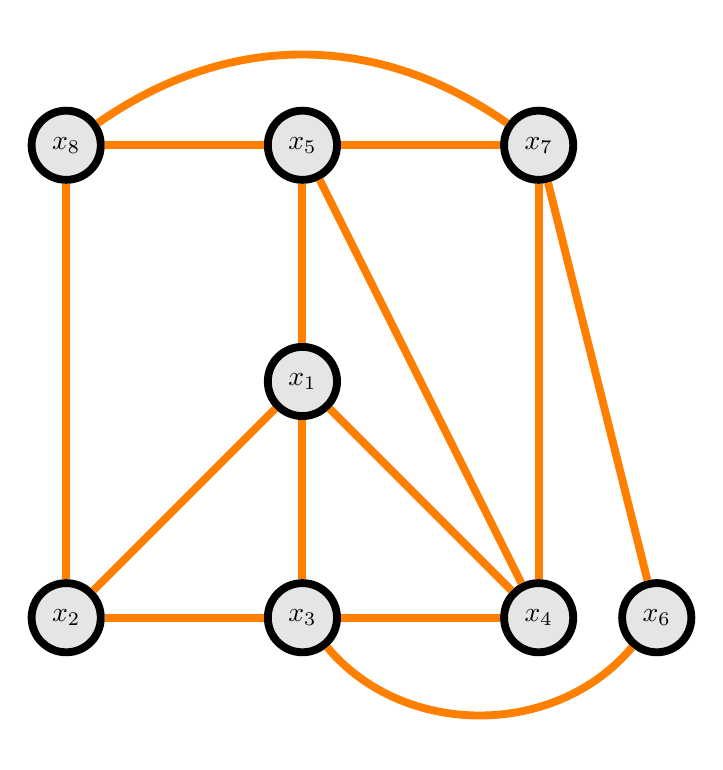
\begin{tikzpicture}[font=\sffamily]
        % Setup the style for the states
        \tikzset{node style/.style={state, 
                                    minimum width=0.5cm,
                                    line width=1mm,
                                    fill=gray!20!white}}
 
        % Draw the states
        \node[node style] at (0, 6)     (bull)     {$x_8$};
        \node[node style] at (3, 3)     (bear)     {$x_1$};
        \node[node style] at (3, 6) (stagnant) {$x_5$};
        \node[node style] at (6, 6) (masha) {$x_7$};
        \node[node style] at (0,0) (masha2) {$x_2$};
        \node[node style] at (3,0) (masha3) {$x_3$};
        \node[node style] at (6,0) (masha4) {$x_4$};
        \node[node style] at (7.5,0) (masha5) {$x_6$};
        % Connect the states with arrows
        \draw[
              line width=1mm,
              draw=orange,
              fill=orange]
            (stagnant)     edge[bend right=0]            node {} (masha)
            (stagnant)     edge[bend left=0]            node {} (bear)
            (bull)     edge[bend left=0]            node {} (stagnant)
            (bull)     edge[bend left=0]            node {} (masha2)
            (bull)     edge[bend left=35]            node {} (masha)
            (stagnant)     edge[bend right=0]            node {} (masha4)
            (bear)     edge[bend right=0]            node {} (masha2)
            (bear)     edge[bend right=0]            node {} (masha4)
            (masha3)     edge[bend right=0]            node {} (masha2)
            (masha3)     edge[bend right=0]            node {} (bear)
            (masha3)     edge[bend right=0]            node {} (masha4)
            (masha4)     edge[bend right=0]            node {} (masha)
            (masha5)     edge[bend left=50]            node {} (masha3)
            (masha5)     edge[bend right=0]            node {} (masha);
\end{tikzpicture}
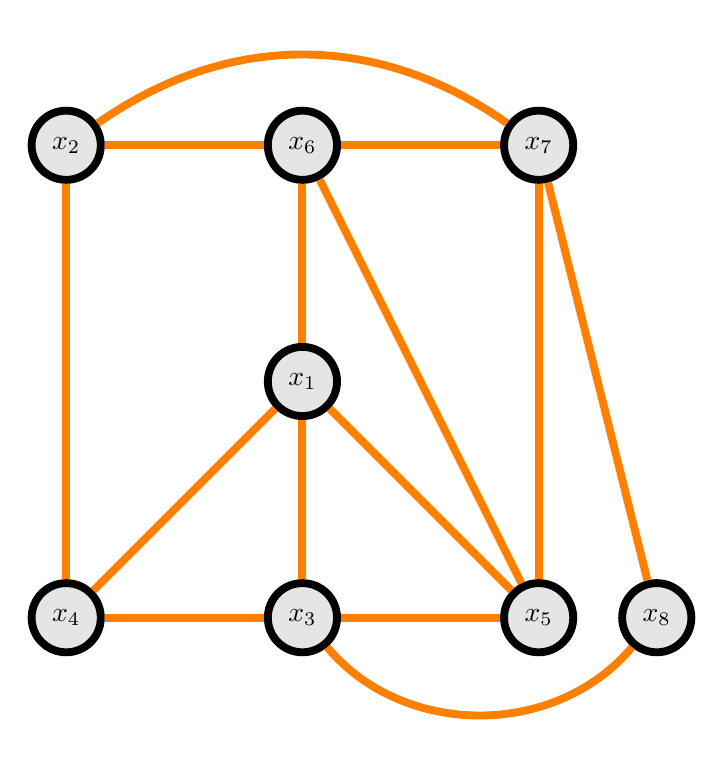
\begin{tikzpicture}[font=\sffamily]
        % Setup the style for the states
        \tikzset{node style/.style={state, 
                                    minimum width=0.5cm,
                                    line width=1mm,
                                    fill=gray!20!white}}
 
        % Draw the states
        \node[node style] at (0, 6)     (bull)     {$x_2$};
        \node[node style] at (3, 3)     (bear)     {$x_1$};
        \node[node style] at (3, 6) (stagnant) {$x_6$};
        \node[node style] at (6, 6) (masha) {$x_7$};
        \node[node style] at (0,0) (masha2) {$x_4$};
        \node[node style] at (3,0) (masha3) {$x_3$};
        \node[node style] at (6,0) (masha4) {$x_5$};
        \node[node style] at (7.5,0) (masha5) {$x_8$};
        % Connect the states with arrows
        \draw[
              line width=1mm,
              draw=orange,
              fill=orange]
            (stagnant)     edge[bend right=0]            node {} (masha)
            (stagnant)     edge[bend left=0]            node {} (bear)
            (bull)     edge[bend left=0]            node {} (stagnant)
            (bull)     edge[bend left=0]            node {} (masha2)
            (bull)     edge[bend left=35]            node {} (masha)
            (stagnant)     edge[bend right=0]            node {} (masha4)
            (bear)     edge[bend right=0]            node {} (masha2)
            (bear)     edge[bend right=0]            node {} (masha4)
            (masha3)     edge[bend right=0]            node {} (masha2)
            (masha3)     edge[bend right=0]            node {} (bear)
            (masha3)     edge[bend right=0]            node {} (masha4)
            (masha4)     edge[bend right=0]            node {} (masha)
            (masha5)     edge[bend left=50]            node {} (masha3)
            (masha5)     edge[bend right=0]            node {} (masha);
\end{tikzpicture}
\\
c) Utvrdimo planarnost grafova: \\
\\
- Grafovi $G_1$ odnosno $G_3$ su planarni (prijašnje slike). \\
\\
- Za graf $G_2$ se međutim ne vidi očigledan način da se nacrta bez presijecanja grana. Na osnovu
Eulerove teoreme, slijedi da planaran graf sa n čvorova može imati najviše 3 ${\cdot}$ n – 6 grana. U ovom
slučaju, uslov je zadovoljen jer je 3 ${\cdot}$ 8 – 6 = 24 – 6 = 18, a razmatrani graf ima 14 grana, što znači
da je potreban uslov planaranosti ispunjen. Za provjeru da li graf zaista jeste planaran bit će
korištena Wagnerova teorema, tačnije svođenje grafa na $K_5$. Ako primjetimo možemo utapanjem čvorova $x_1$ u $x_7$, $x_6$ u $x_5$, $x_3$ u $x_4$ dobiti sljedeći graf, koji je očigledno $K_5$ samim tim naš graf $G_2$ nije planaran (grafik $G_2$ je ilustrovan u pod d) - desni). \\

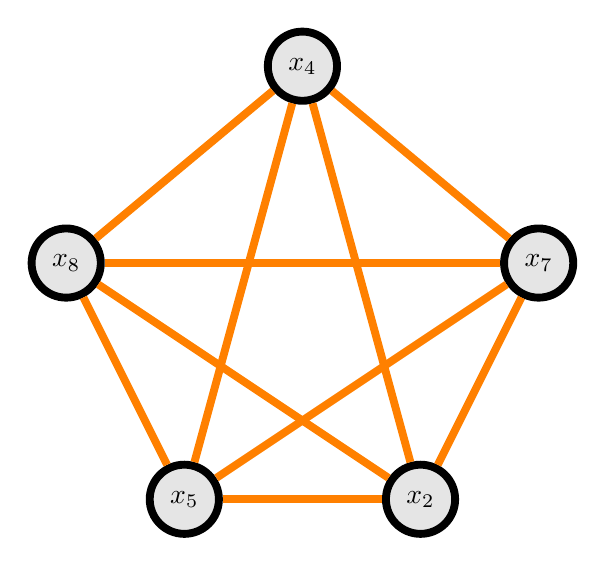
\begin{tikzpicture}[font=\sffamily]
        % Setup the style for the states
        \tikzset{node style/.style={state, 
                                    minimum width=0.5cm,
                                    line width=1mm,
                                    fill=gray!20!white}}
 
        % Draw the states
        \node[node style] at (3, 5.5) (masha4) {$x_4$};
        \node[node style] at (0, 3) (masha8) {$x_8$};
        \node[node style] at (6, 3) (masha7) {$x_7$};
        \node[node style] at (1.5, 0) (masha5) {$x_5$};
        \node[node style] at (4.5, 0) (masha2) {$x_2$};
        % Connect the states with arrows
        \draw[
              line width=1mm,
              draw=orange,
              fill=orange]
              (masha4)     edge[bend right=0]            node {} (masha8)
              (masha4)     edge[bend right=0]            node {} (masha7)
              (masha4)     edge[bend right=0]            node {} (masha5)
              (masha4)     edge[bend right=0]            node {} (masha2)
              (masha8)     edge[bend right=0]            node {} (masha5)
              (masha8)     edge[bend right=0]            node {} (masha2)
              (masha8)     edge[bend right=0]            node {} (masha7)
              (masha5)     edge[bend right=0]            node {} (masha2)
              (masha5)     edge[bend right=0]            node {} (masha7)
              (masha2)     edge[bend right=0]            node {} (masha7);
\end{tikzpicture}
\\
\\
d) Hromatski broj planarnih grafova uvijek je manji ili jednak od 4. Ukoliko se bojenje vrši
pohlepnim algoritmom, situacija je sljedeća za $G_1$ odnosno $G_3$ (isto bojanje) na lijevom grafu, odnoso $G_2$ na desnom: \\
\\
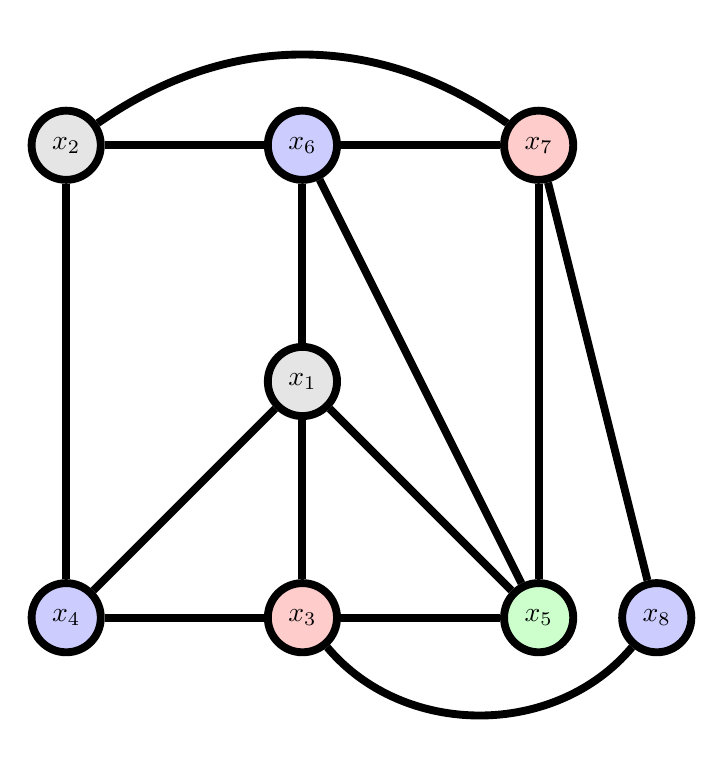
\begin{tikzpicture}[font=\sffamily]
        % Setup the style for the states
        \tikzset{node style/.style={state, 
                                    minimum width=0.5cm,
                                    line width=1mm,
                                    fill=gray!20!white}}
        \tikzset{node style2/.style={state, 
                                    minimum width=0.5cm,
                                    line width=1mm,
                                    fill=blue!20!white}}
        \tikzset{node style3/.style={state, 
                                    minimum width=0.5cm,
                                    line width=1mm,
                                    fill=red!20!white}}
        \tikzset{node style4/.style={state, 
                                    minimum width=0.5cm,
                                    line width=1mm,
                                    fill=green!20!white}}
 
        % Draw the states
        \node[node style] at (0, 6)     (bull)     {$x_2$};
        \node[node style] at (3, 3)     (bear)     {$x_1$};
        \node[node style2] at (3, 6) (stagnant) {$x_6$};
        \node[node style3] at (6, 6) (masha) {$x_7$};
        \node[node style2] at (0,0) (masha2) {$x_4$};
        \node[node style3] at (3,0) (masha3) {$x_3$};
        \node[node style4] at (6,0) (masha4) {$x_5$};
        \node[node style2] at (7.5,0) (masha5) {$x_8$};
        % Connect the states with arrows
        \draw[
              line width=1mm,
              draw=black,
              fill=black]
            (stagnant)     edge[bend right=0]            node {} (masha)
            (stagnant)     edge[bend left=0]            node {} (bear)
            (bull)     edge[bend left=0]            node {} (stagnant)
            (bull)     edge[bend left=0]            node {} (masha2)
            (bull)     edge[bend left=35]            node {} (masha)
            (stagnant)     edge[bend right=0]            node {} (masha4)
            (bear)     edge[bend right=0]            node {} (masha2)
            (bear)     edge[bend right=0]            node {} (masha4)
            (masha3)     edge[bend right=0]            node {} (masha2)
            (masha3)     edge[bend right=0]            node {} (bear)
            (masha3)     edge[bend right=0]            node {} (masha4)
            (masha4)     edge[bend right=0]            node {} (masha)
            (masha5)     edge[bend left=50]            node {} (masha3)
            (masha5)     edge[bend right=0]            node {} (masha);
\end{tikzpicture}
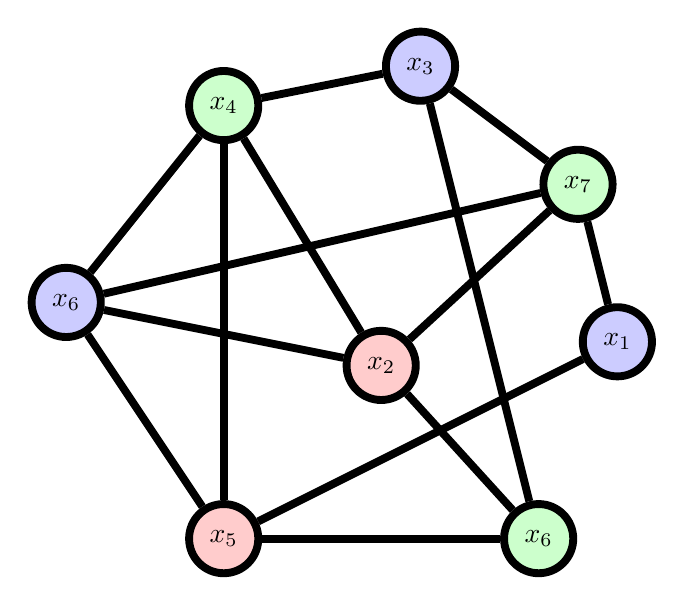
\begin{tikzpicture}[font=\sffamily]
        % Setup the style for the states
        \tikzset{node style/.style={state, 
                                    minimum width=0.5cm,
                                    line width=1mm,
                                    fill=gray!20!white}}
        \tikzset{node style2/.style={state, 
                                    minimum width=0.5cm,
                                    line width=1mm,
                                    fill=blue!20!white}}
        \tikzset{node style3/.style={state, 
                                    minimum width=0.5cm,
                                    line width=1mm,
                                    fill=red!20!white}}
        \tikzset{node style4/.style={state, 
                                    minimum width=0.5cm,
                                    line width=1mm,
                                    fill=green!20!white}}
 
        % Draw the states
        \node[node style4] at (2, 5.5) (masha4) {$x_4$};
        \node[node style2] at (4.5, 6) (masha3) {$x_3$};
        \node[node style2] at (0, 3) (masha8) {$x_6$};
        \node[node style4] at (6.5, 4.5) (masha7) {$x_7$};
        \node[node style3] at (2, 0) (masha5) {$x_5$};
        \node[node style3] at (4, 2.2) (masha2) {$x_2$};
        \node[node style4] at (6,0) (masha6) {$x_6$};
        \node[node style2] at (7, 2.5) (masha1) {$x_1$};
        % Connect the states with arrows
        \draw[
              line width=1mm,
              draw=black,
              fill=black]
              (masha4)     edge[bend right=0]            node {} (masha8)
              (masha4)     edge[bend right=0]            node {} (masha3)
              (masha3)     edge[bend right=0]            node {} (masha7)
              (masha4)     edge[bend right=0]            node {} (masha5)
              (masha4)     edge[bend right=0]            node {} (masha2)
              (masha8)     edge[bend right=0]            node {} (masha5)
              (masha8)     edge[bend right=0]            node {} (masha2)
              (masha8)     edge[bend right=0]            node {} (masha7)
              (masha5)     edge[bend right=0]            node {} (masha6)
              (masha2)     edge[bend right=0]            node {} (masha7)
              (masha1)     edge[bend right=0]            node {} (masha5)
              (masha1)     edge[bend right=0]            node {} (masha7)
              (masha2)     edge[bend right=0]            node {} (masha6)
              (masha3)     edge[bend right=0]            node {} (masha6);
\end{tikzpicture}
\\
Bojimo $x_2$ sa sivom, zatim $x_4$ sa plavom, onda $x_1$ opet sivom, dalje $x_6$ bojimo opet plavom. $x_7$ bojimo novom bojom, jer ne možemo sa plavom i sivom. Dalje $x_8$ možemo plavom opet. $x_3$ moramo crvenom jer je povezan sa čvorovima sive i plave boje. Na kraju $x_5$ bojimo sa novom bojom, tj. zelenom, jer već postojeće 3 boje ne možemo izabrati. Time dobijamo da je hromatski broj ovih grafova 4.
\\
\\
Bojenje $G_2$ smo uradili na isti način prolaskom redom kroz $x_6 - x_4 - x_3 - x_7 - x_1 - x_5 - x_6 - x_2$. Time dobijamo da je hromatski broj grafa $G_2$ 3.
\newpage

\item Rješenje zadatka \\
		\\
		Zadatak 2 [0.6 poena] \\
		\\
		a) Primjenom Kruskalovog algoritma sa bojenjem čvorova:
		\\
		\\
		\begin{tabular}{|c|c|c|c|c|c|c|c|c|c|c|c|c|c|c|}
\hline
Grana & Težina & Uzeti & $c_1$ & $c_2$ & $c_3$ & $c_4$ & $c_5$ & $c_6$ & $c_7$ & $c_8$ & $c_9$ & $c_{10}$ & $c_{11}$ & $c_{12}$ \\ \hline
4-10  & 250    & da    &       &       &       & 1     &       &       &       &       &       & 1        &          &          \\ \hline
5-10  & 270    & da    &       &       &       &       & 1     &       &       &       &       &          &          &          \\ \hline
3-6   & 330    & da    &       &       & 2     &       &       & 2     &       &       &       &          &          &          \\ \hline
3-7   & 400    & da    &       &       &       &       &       &       & 2     &       &       &          &          &          \\ \hline
4-8   & 420    & da    &       &       &       &       &       &       &       & 1     &       &          &          &          \\ \hline
3-5   & 480    & da    &       &       & 1     &       &       & 1     & 1     &       &       &          &          &          \\ \hline
1-4   & 620    & da    & 1     &       &       &       &       &       &       &       &       &          &          &          \\ \hline
3-4   & 690    & ne    &       &       &       &       &       &       &       &       &       &          &          &          \\ \hline
2-6   & 730    & da    &       & 1     &       &       &       &       &       &       &       &          &          &          \\ \hline
2-7   & 810    & ne    &       &       &       &       &       &       &       &       &       &          &          &          \\ \hline
1-5   & 810    & ne    &       &       &       &       &       &       &       &       &       &          &          &          \\ \hline
1-10  & 840    & ne    &       &       &       &       &       &       &       &       &       &          &          &          \\ \hline
11-12 & 840    & da    &       &       &       &       &       &       &       &       &       &          & 3        & 3        \\ \hline
3-12  & 950    & da    &       &       &       &       &       &       &       &       &       &          & 1        & 1        \\ \hline
1-3   & 960    & ne    &       &       &       &       &       &       &       &       &       &          &          &          \\ \hline
9-12  & 1040   & da    &       &       &       &       &       &       &       &       & 1     &          &          &          \\ \hline
\end{tabular}
    \\
    \\
    b) Primjenom optimalnog Kruskalovog algoritma:
	\\
	\\
	\scalebox{0.9}{
	\begin{tabular}{|c|c|c|c|c|c|c|c|c|c|c|c|c|c|c|}
\hline
Grana & Težina & Uzeti & $x_1/1$ & $x_2/1$ & $x_3/1$ & $x_4/1$  & $x_5/1$    & $x_6/1$ & $x_7/1$ & $x_8/1$ & $x_9/1$    & $x_{10}/1$ & $x_{11}/1$ & $x_{12}/1$ \\ \hline
4-10  & 250    & da    &         &         &         & $x_4/2$  &            &         &         &         &            & $x_4/1$    &            &            \\ \hline
5-10  & 270    & da    &         &         &         & $x_4/3$  & $x_{10}/1$ &         &         &         &            &            &            &            \\ \hline
3-6   & 330    & da    &         &         & $x_3/2$ &          &            & $x_3/1$ &         &         &            &            &            &            \\ \hline
3-7   & 400    & da    &         &         & $x_3/3$ &          &            &         & $x_3/1$ &         &            &            &            &            \\ \hline
4-8   & 420    & da    &         &         &         & $x_4/4$  &            &         &         & $x_4/1$ &            &            &            &            \\ \hline
3-5   & 480    & da    &         &         & $x_5/3$ & $x_4/7$  &            &         &         &         &            &            &            &            \\ \hline
1-4   & 620    & da    & $x_4/1$ &         &         & $x_4/8$  &            &         &         &         &            &            &            &            \\ \hline
3-4   & 690    & ne    &         &         &         &          &            &         &         &         &            &            &            &            \\ \hline
2-6   & 730    & da    &         & $x_6/1$ &         & $x_4/9$  &            &         &         &         &            &            &            &            \\ \hline
2-7   & 810    & ne    &         &         &         &          &            &         &         &         &            &            &            &            \\ \hline
1-5   & 810    & ne    &         &         &         &          &            &         &         &         &            &            &            &            \\ \hline
1-10  & 840    & ne    &         &         &         &          &            &         &         &         &            &            &            &            \\ \hline
11-12 & 840    & da    &         &         &         &          &            &         &         &         &            &            & $x_{11}/2$ & $x_{11}/1$ \\ \hline
3-12  & 950    & da    &         &         &         & $x_4/11$ &            &         &         &         &            &            & $x_3/2$    &            \\ \hline
1-3   & 960    & ne    &         &         &         &          &            &         &         &         &            &            &            &            \\ \hline
9-12  & 1040   & da    &         &         &         & $x_4/12$ &            &         &         &         & $x_{12}/1$ &            &            &            \\ \hline
\end{tabular}
	}
	\\
	\\
	c) Primjenom optimiziranog (kvadratnog) Primovog algoritma: \\
	\newpage
	\scalebox{0.85}{
	\begin{tabular}{|c|c|c|c|c|c|c|c|c|c|c|c|c|}
\hline
$x_r$    & 1                                 & 2                                & 3                                & 4                                & 5                                   & 6                                & 7                                & 8                                & 9                                    & 10                               & 11                                  & 12                               \\ \cline{2-13} 
         & {\color[HTML]{FE0000} \textbf{0}} & -                                & -                                & -                                & -                                   & -                                & -                                & -                                & -                                    & -                                & -                                   & -                                \\ \hline
$x_1$    &                                   &                                  & $960/x_1$                        & {\color[HTML]{FE0000} $620/x_1$} & $810/x_1$                           &                                  &                                  &                                  & $1170/x_1$                           & $840/x_1$                        &                                     &                                  \\ \hline
$x_4$    &                                   &                                  & $690/x_4$                        &                                  & $810/x_1$                           &                                  &                                  & $420/x_4$                        & $1170/x_1$                           & {\color[HTML]{FE0000} $250/x_4$} &                                     &                                  \\ \hline
$x_{10}$ &                                   &                                  & $690/x_4$                        &                                  & {\color[HTML]{FE0000} $270/x_{10}$} &                                  &                                  & $420/x_4$                        & $1170/x_1$                           &                                  &                                     &                                  \\ \hline
$x_5$    &                                   &                                  & $480/x_5$                        &                                  & \textbf{}                           & $1100/x_5$                       &                                  & {\color[HTML]{FE0000} $420/x_4$} & $1090/x_5$                           &                                  &                                     &                                  \\ \hline
$x_8$    &                                   &                                  & {\color[HTML]{FE0000} $480/x_5$} &                                  &                                     & $1100/x_5$                       &                                  &                                  & $1090/x_5$                           &                                  &                                     &                                  \\ \hline
$x_3$    & {\color[HTML]{000000} }           &                                  & \textbf{}                        &                                  &                                     & {\color[HTML]{FE0000} $330/x_3$} & $400/x_3$                        &                                  & $1090/x_5$                           &                                  & $1370/x_3$                          & $950/x_3$                        \\ \hline
$x_6$    &                                   & $730/x_6$                        &                                  &                                  &                                     &                                  & {\color[HTML]{CB0000} $400/x_3$} &                                  & {\color[HTML]{000000} $1090/x_5$}    &                                  & $1370/x_3$                          & $950/x_3$                        \\ \hline
$x_7$    & {\color[HTML]{FE0000} }           & {\color[HTML]{FE0000} $730/x_6$} &                                  &                                  &                                     & {\color[HTML]{FE0000} }          & \textbf{}                        &                                  & $1090/x_5$                           &                                  & $1370/x_3$                          & $950/x_3$                        \\ \hline
$x_2$    &                                   & {\color[HTML]{FE0000} }          &                                  &                                  &                                     &                                  &                                  &                                  & $1090/x_5$                           &                                  & $1370/x_3$                          & {\color[HTML]{FE0000} $950/x_3$} \\ \hline
$x_{12}$ &                                   &                                  &                                  &                                  &                                     &                                  &                                  & \textbf{}                        & {\color[HTML]{000000} $1040/x_{12}$} &                                  & {\color[HTML]{FE0000} $840/x_{12}$} & {\color[HTML]{FE0000} }          \\ \hline
$x_{11}$ &                                   &                                  &                                  &                                  &                                     &                                  &                                  &                                  & {\color[HTML]{FE0000} $1040/x_{12}$} &                                  & {\color[HTML]{FE0000} }             &                                  \\ \hline
\end{tabular}
}
\\
\\
\\
\item Rješenje zadatka \\
\\
Zadatak 3 [0.7 poena] \\
\\
Označavamo gradove slovima abecede, radi lakšeg rada sa imenima
čvorova: A-Rekazga, B-Zixa, C-Evesa, D-Egna, E-Quwuti, F-Brot, G-
Zote, H-Uhsuru.
\\
\\
A - Rekazga
\\
\\
\begin{tabular}{|c|c|c|c|c|c|c|c|c|}
\hline
Cvor ($x_r$) & A                        & B                            & C                            & D                            & E                            & F                            & G                            & H                            \\ \cline{2-9} 
             & {\color[HTML]{FE0000} 0} & -                            & -                            & -                            & -                            & -                            & -                            & -                            \\ \hline
A (0)        &                          & 1430/A                       &                              & 1410/A                       & {\color[HTML]{FE0000} 220/A} &                              & 390/A                        & 250/A                        \\ \hline
E (220)      &                          & 1370/E                       & 1450/E                       & 1410/A                       &                              & 550/E                        & 390/A                        & {\color[HTML]{FE0000} 250/A} \\ \hline
H (250)      &                          & 1200/H                       & 1130/E                       & 740/H                        &                              & 550/E                        & {\color[HTML]{FE0000} 390/A} &                              \\ \hline
G (390)      &                          & 820/G                        & {\color[HTML]{000000} 690/G} & {\color[HTML]{000000} 630/G} &                              & {\color[HTML]{FE0000} 550/E} &                              &                              \\ \hline
F (550)      &                          & 820/G                        & {\color[HTML]{000000} 690/G} & {\color[HTML]{FE0000} 630/G} &                              &                              &                              &                              \\ \hline
D (630)      &                          & 820/G                        & {\color[HTML]{FE0000} 690/G} & {\color[HTML]{FE0000} }      &                              &                              &                              &                              \\ \hline
C (690)      &                          & {\color[HTML]{FE0000} 820/G} &                              &                              &                              &                              &                              &                              \\ \hline
\end{tabular}
\\
\\
B - Zixa
\\
\\
\begin{tabular}{|c|c|c|c|c|c|c|c|c|}
\hline
Cvor ($x_r$) & A                            & B                        & C                            & D                            & E                             & F                            & G                            & H                            \\ \cline{2-9} 
             & {\color[HTML]{000000} -}     & {\color[HTML]{FE0000} 0} & -                            & -                            & -                             & -                            & -                            & -                            \\ \hline
B (0)        & 1430/B                       &                          & 1090/B                       & 1480/B                       & {\color[HTML]{333333} 1150/B} & 540/B                        & {\color[HTML]{FE0000} 430/B} & 950/B                        \\ \hline
G (430)      & 820/G                        &                          & 730/G                        & 670/G                        & 790/G                         & {\color[HTML]{FE0000} 540/B} &                              & {\color[HTML]{333333} 690/G} \\ \hline
F (540)      & 820/G                        &                          & 730/G                        & {\color[HTML]{FE0000} 670/G} & 790/G                         &                              & {\color[HTML]{FE0000} }      & 690/G                        \\ \hline
D (670)      & 820/G                        &                          & {\color[HTML]{000000} 730/G} & {\color[HTML]{000000} }      & 790/G                         & {\color[HTML]{FE0000} }      &                              & {\color[HTML]{FE0000} 690/G} \\ \hline
H (690)      & 820/G                        &                          & {\color[HTML]{FE0000} 730/G} & {\color[HTML]{FE0000} }      & 790/G                         &                              &                              &                              \\ \hline
C (730)      & 820/G                        &                          & {\color[HTML]{FE0000} }      & {\color[HTML]{FE0000} }      & {\color[HTML]{FE0000} 790/G}  &                              &                              &                              \\ \hline
E (790)      & {\color[HTML]{FE0000} 820/G} & {\color[HTML]{FE0000} }  &                              &                              &                               &                              &                              &                              \\ \hline
\end{tabular}
\newpage
C - Evesa
\\
\\
\begin{tabular}{|c|c|c|c|c|c|c|c|c|}
\hline
Cvor ($x_r$) & A                            & B                            & C                        & D                            & E                             & F                            & G                            & H                            \\ \cline{2-9} 
             & {\color[HTML]{000000} -}     & {\color[HTML]{333333} -}     & {\color[HTML]{FE0000} 0} & -                            & -                             & -                            & -                            & -                            \\ \hline
C (0)        &                              & 1090/C                       &                          &                              & {\color[HTML]{333333} 1230/C} & {\color[HTML]{FE0000} 220/C} & {\color[HTML]{333333} 300/C} & 880/C                        \\ \hline
F (220)      &                              & 760/F                        &                          & 580/F                        & 550/F                         & {\color[HTML]{FE0000} }      & {\color[HTML]{FE0000} 300/C} & {\color[HTML]{333333} 530/F} \\ \hline
G (300)      & 690/G                        & 730/G                        &                          & {\color[HTML]{333333} 540/G} & 550/F                         &                              & {\color[HTML]{FE0000} }      & {\color[HTML]{FE0000} 530/F} \\ \hline
F (530)      & 690/G                        & 730/G                        & {\color[HTML]{000000} }  & {\color[HTML]{FE0000} 540/G} & 550/F                         & {\color[HTML]{FE0000} }      &                              & {\color[HTML]{FE0000} }      \\ \hline
D (540)      & 690/G                        & 730/G                        & {\color[HTML]{FE0000} }  & {\color[HTML]{FE0000} }      & {\color[HTML]{FE0000} 550/F}  &                              &                              &                              \\ \hline
E (550)      & {\color[HTML]{FE0000} 690/G} & 730/G                        & {\color[HTML]{FE0000} }  & {\color[HTML]{FE0000} }      & {\color[HTML]{FE0000} }       &                              &                              &                              \\ \hline
A (690)      & {\color[HTML]{FE0000} }      & {\color[HTML]{FE0000} 730/G} &                          &                              &                               &                              &                              &                              \\ \hline
\end{tabular}
\\
\\
D - Egna
\\
\\
\begin{tabular}{|c|c|c|c|c|c|c|c|c|}
\hline
Cvor ($x_r$) & A                            & B                            & C                            & D                        & E                             & F                            & G                            & H                            \\ \cline{2-9} 
             & {\color[HTML]{000000} -}     & {\color[HTML]{333333} -}     & -                            & {\color[HTML]{FE0000} 0} & -                             & -                            & -                            & -                            \\ \hline
D (0)        & 1410/D                       & 1480/D                       &                              &                          & {\color[HTML]{333333} 1490/D} & 360/D                        & {\color[HTML]{FE0000} 240/D} & 490/D                        \\ \hline
G (240)      & 630/G                        & 670/G                        & 540/G                        &                          & 600/G                         & {\color[HTML]{FE0000} 360/D} &                              & {\color[HTML]{333333} 490/D} \\ \hline
F (360)      & 630/G                        & 670/G                        & 540/G                        & {\color[HTML]{FE0000} }  & 600/G                         &                              & {\color[HTML]{FE0000} }      & {\color[HTML]{FE0000} 490/D} \\ \hline
H (490)      & 630/G                        & 670/G                        & {\color[HTML]{FE0000} 540/G} & {\color[HTML]{000000} }  & 600/G                         & {\color[HTML]{FE0000} }      &                              & {\color[HTML]{FE0000} }      \\ \hline
C (540)      & 630/G                        & 670/G                        & {\color[HTML]{FE0000} }      & {\color[HTML]{FE0000} }  & {\color[HTML]{FE0000} 600/G}  &                              &                              &                              \\ \hline
E (600)      & {\color[HTML]{FE0000} 630/G} & 670/G                        & {\color[HTML]{FE0000} }      & {\color[HTML]{FE0000} }  & {\color[HTML]{FE0000} }       &                              &                              &                              \\ \hline
A (630)      & {\color[HTML]{FE0000} }      & {\color[HTML]{FE0000} 670/G} &                              &                          &                               &                              &                              &                              \\ \hline
\end{tabular}
\\
\\
E - Quwuti
\\
\\
\begin{tabular}{|c|c|c|c|c|c|c|c|c|}
\hline
Cvor ($x_r$) & A                            & B                            & C                            & D                            & E                        & F                            & G                            & H                            \\ \cline{2-9} 
             & {\color[HTML]{000000} -}     & {\color[HTML]{333333} -}     & -                            & {\color[HTML]{000000} -}     & {\color[HTML]{FE0000} 0} & -                            & -                            & -                            \\ \hline
E (0)        & {\color[HTML]{FE0000} 220/E} & 1150/E                       & 1230/E                       & 1490/E                       & {\color[HTML]{333333} }  & 330/E                        & {\color[HTML]{333333} 360/E} &                              \\ \hline
A (220)      &                              & 1150/E                       & 1230/E                       & 1490/E                       &                          & {\color[HTML]{FE0000} 330/E} & 360/E                        & {\color[HTML]{333333} 470/A} \\ \hline
F (330)      &                              & 870/F                        & 550/F                        & {\color[HTML]{333333} 690/F} &                          &                              & {\color[HTML]{FE0000} 360/E} & {\color[HTML]{333333} 470/A} \\ \hline
G (360)      &                              & 790/G                        & {\color[HTML]{333333} 550/F} & {\color[HTML]{000000} 600/G} &                          & {\color[HTML]{FE0000} }      &                              & {\color[HTML]{FE0000} 470/A} \\ \hline
H (470)      &                              & 790/G                        & {\color[HTML]{FE0000} 550/F} & {\color[HTML]{333333} 600/G} & {\color[HTML]{FE0000} }  &                              &                              &                              \\ \hline
C (550)      & {\color[HTML]{FE0000} }      & 790/G                        & {\color[HTML]{FE0000} }      & {\color[HTML]{FE0000} 600/G} & {\color[HTML]{FE0000} }  &                              &                              &                              \\ \hline
G (600)      & {\color[HTML]{FE0000} }      & {\color[HTML]{FE0000} 790/G} &                              &                              &                          &                              &                              &                              \\ \hline
\end{tabular}
\\
\\
F - Brot
\\
\\
\begin{tabular}{|c|c|c|c|c|c|c|c|c|}
\hline
Cvor ($x_r$) & A                            & B                            & C                            & D                            & E                            & F                        & G                            & H                            \\ \cline{2-9} 
             & {\color[HTML]{000000} -}     & {\color[HTML]{333333} -}     & {\color[HTML]{333333} -}     & -                            & -                            & {\color[HTML]{FE0000} 0} & -                            & -                            \\ \hline
F (0)        &                              & 540/F                        & {\color[HTML]{FE0000} 220/F} & 360/F                        & {\color[HTML]{333333} 330/F} & {\color[HTML]{FE0000} }  & {\color[HTML]{333333} 460/F} & 310/F                        \\ \hline
C (220)      &                              & 540/F                        &                              & 360/F                        & 330/F                        & {\color[HTML]{FE0000} }  & {\color[HTML]{333333} 460/F} & {\color[HTML]{FE0000} 310/F} \\ \hline
H (310)      & 560/H                        & 540/F                        &                              & {\color[HTML]{333333} 360/F} & {\color[HTML]{FE0000} 330/F} &                          & {\color[HTML]{333333} 460/F} & {\color[HTML]{FE0000} }      \\ \hline
E (330)      & 550/E                        & 540/F                        & {\color[HTML]{000000} }      & {\color[HTML]{FE0000} 360/F} &                              & {\color[HTML]{FE0000} }  & {\color[HTML]{333333} 460/F} & {\color[HTML]{FE0000} }      \\ \hline
D (360)      & 550/E                        & {\color[HTML]{333333} 540/F} & {\color[HTML]{FE0000} }      & {\color[HTML]{FE0000} }      & {\color[HTML]{FE0000} }      &                          & {\color[HTML]{FE0000} 460/F} &                              \\ \hline
G (460)      & {\color[HTML]{333333} 550/E} & {\color[HTML]{FE0000} 540/F} & {\color[HTML]{FE0000} }      & {\color[HTML]{FE0000} }      & {\color[HTML]{FE0000} }      &                          &                              &                              \\ \hline
B (540)      & {\color[HTML]{FE0000} 550/E} & {\color[HTML]{FE0000} }      &                              &                              &                              &                          &                              &                              \\ \hline
\end{tabular}
\newpage
G - Zote
\\
\\
\begin{tabular}{|c|c|c|c|c|c|c|c|c|}
\hline
Cvor ($x_r$) & A                            & B                            & C                            & D                            & E                            & F                            & G                        & H                            \\ \cline{2-9} 
             & {\color[HTML]{000000} -}     & {\color[HTML]{333333} -}     & {\color[HTML]{333333} -}     & -                            & -                            & {\color[HTML]{333333} -}     & {\color[HTML]{FE0000} 0} & -                            \\ \hline
G (0)        & 390/G                        & 430/G                        & {\color[HTML]{333333} 300/G} & {\color[HTML]{FE0000} 240/G} & {\color[HTML]{333333} 360/G} & {\color[HTML]{333333} 460/G} & {\color[HTML]{333333} }  & 260/G                        \\ \hline
D (240)      & 390/G                        & 430/G                        & 300/G                        &                              & 360/G                        & {\color[HTML]{333333} 460/G} & {\color[HTML]{333333} }  & {\color[HTML]{FE0000} 260/G} \\ \hline
H (260)      & 390/G                        & 430/G                        & {\color[HTML]{FE0000} 300/G} & {\color[HTML]{333333} }      & {\color[HTML]{333333} 360/G} & 460/G                        & {\color[HTML]{333333} }  & {\color[HTML]{FE0000} }      \\ \hline
C (300)      & 390/G                        & 430/G                        & {\color[HTML]{000000} }      & {\color[HTML]{FE0000} }      & {\color[HTML]{FE0000} 360/G} & {\color[HTML]{333333} 460/G} & {\color[HTML]{333333} }  & {\color[HTML]{FE0000} }      \\ \hline
E (360)      & {\color[HTML]{FE0000} 390/G} & {\color[HTML]{333333} 430/G} & {\color[HTML]{FE0000} }      & {\color[HTML]{FE0000} }      & {\color[HTML]{FE0000} }      & 460/G                        & {\color[HTML]{FE0000} }  &                              \\ \hline
A (390)      & {\color[HTML]{333333} }      & {\color[HTML]{FE0000} 430/G} & {\color[HTML]{FE0000} }      & {\color[HTML]{FE0000} }      & {\color[HTML]{FE0000} }      & 460/G                        &                          &                              \\ \hline
B (430)      & {\color[HTML]{FE0000} }      & {\color[HTML]{FE0000} }      &                              &                              &                              & {\color[HTML]{FE0000} 460/G} &                          &                              \\ \hline
\end{tabular}
\\
\\
H - Uhsuru
\\
\\
\begin{tabular}{|c|c|c|c|c|c|c|c|c|}
\hline
Cvor ($x_r$) & A                            & B                            & C                            & D                            & E                            & F                            & G                            & H                        \\ \cline{2-9} 
             & {\color[HTML]{000000} -}     & {\color[HTML]{333333} -}     & {\color[HTML]{333333} -}     & -                            & -                            & {\color[HTML]{333333} -}     & {\color[HTML]{333333} -}     & {\color[HTML]{FE0000} 0} \\ \hline
H (0)        & {\color[HTML]{FE0000} 250/H} & 950/H                        & {\color[HTML]{333333} 880/H} & {\color[HTML]{333333} 490/H} & {\color[HTML]{333333} }      & {\color[HTML]{333333} 310/H} & {\color[HTML]{333333} 260/H} &                          \\ \hline
A (250)      &                              & 950/H                        & 880/H                        & 490/H                        & 470/A                        & {\color[HTML]{333333} 310/H} & {\color[HTML]{FE0000} 260/H} & {\color[HTML]{FE0000} }  \\ \hline
G (260)      &                              & 690/G                        & {\color[HTML]{333333} 560/G} & {\color[HTML]{333333} 490/H} & {\color[HTML]{333333} 470/A} & {\color[HTML]{FE0000} 310/H} & {\color[HTML]{333333} }      & {\color[HTML]{FE0000} }  \\ \hline
F (310)      &                              & 690/G                        & {\color[HTML]{000000} 530/F} & {\color[HTML]{333333} 490/H} & {\color[HTML]{FE0000} 470/A} & {\color[HTML]{333333} }      & {\color[HTML]{333333} }      & {\color[HTML]{FE0000} }  \\ \hline
E (470)      & {\color[HTML]{FE0000} }      & {\color[HTML]{333333} 690/G} & {\color[HTML]{333333} 530/F} & {\color[HTML]{FE0000} 490/H} & {\color[HTML]{FE0000} }      &                              & {\color[HTML]{FE0000} }      &                          \\ \hline
D (490)      & {\color[HTML]{333333} }      & {\color[HTML]{333333} 690/G} & {\color[HTML]{FE0000} 530/F} & {\color[HTML]{FE0000} }      & {\color[HTML]{FE0000} }      &                              &                              &                          \\ \hline
C (530)      & {\color[HTML]{FE0000} }      & {\color[HTML]{FE0000} 690/G} &                              &                              &                              & {\color[HTML]{FE0000} }      &                              &                          \\ \hline
\end{tabular}
\\
\\
\\
Ovim je postupak sprovođenja Dijkstrinog algoritma okončan. U sljedećoj tablici predstavljen je
konačan rezultat, odnosno minimalne cijene putovanja između dvije destinacije uz informacije o
presjedanju (ako je poželjno) u desnom dijelu do cijene.
\\
\\
\begin{tabular}{|c|c|c|c|c|c|c|c|c|}
\hline
Putovanje & A                            & B                            & C                            & D                            & E                            & F                            & G                          & H                            \\ \hline
A    & {\color[HTML]{333333} 0}     & {\color[HTML]{333333} 820/G} & {\color[HTML]{333333} 690/G} & {\color[HTML]{333333} 630/G} & {\color[HTML]{333333} 220}   & {\color[HTML]{333333} 550/E} & {\color[HTML]{333333} 390} & {\color[HTML]{333333} 250}   \\ \hline
B    & {\color[HTML]{333333} 820/G} & {\color[HTML]{333333} 0}     & {\color[HTML]{333333} 730/G} & {\color[HTML]{333333} 670/G} & {\color[HTML]{333333} 790/G} & {\color[HTML]{333333} 540}   & {\color[HTML]{333333} 430} & {\color[HTML]{333333} 690/G} \\ \hline
C    & {\color[HTML]{333333} 690/G} & {\color[HTML]{333333} 730/G} & {\color[HTML]{333333} 0}     & {\color[HTML]{333333} 540/G} & {\color[HTML]{333333} 550/F} & {\color[HTML]{333333} 220}   & {\color[HTML]{333333} 300} & {\color[HTML]{333333} 530/F} \\ \hline
D    & {\color[HTML]{333333} 630/G} & {\color[HTML]{333333} 670/G} & {\color[HTML]{333333} 540/G} & {\color[HTML]{333333} 0}     & {\color[HTML]{333333} 600/G} & {\color[HTML]{333333} 360}   & {\color[HTML]{333333} 240} & {\color[HTML]{333333} 490}   \\ \hline
E    & {\color[HTML]{333333} 220}   & {\color[HTML]{333333} 790/G} & {\color[HTML]{333333} 550/F} & {\color[HTML]{333333} 600/G} & {\color[HTML]{333333} 0}     & {\color[HTML]{333333} 330}   & {\color[HTML]{333333} 360} & {\color[HTML]{333333} 470/A} \\ \hline
F    & {\color[HTML]{333333} 550/E} & {\color[HTML]{333333} 540}   & {\color[HTML]{333333} 220}   & {\color[HTML]{333333} 360}   & {\color[HTML]{333333} 330}   & {\color[HTML]{333333} 0}     & {\color[HTML]{333333} 460} & {\color[HTML]{333333} 310}   \\ \hline
G    & {\color[HTML]{333333} 390}   & {\color[HTML]{333333} 430}   & {\color[HTML]{333333} 300}   & {\color[HTML]{333333} 240}   & {\color[HTML]{333333} 360}   & {\color[HTML]{333333} 460}   & {\color[HTML]{333333} 0}   & {\color[HTML]{333333} 260}   \\ \hline
H    & {\color[HTML]{333333} 250}   & {\color[HTML]{333333} 690/G} & {\color[HTML]{333333} 530/F} & {\color[HTML]{333333} 490}   & {\color[HTML]{333333} 470/A} & {\color[HTML]{333333} 310}   & {\color[HTML]{333333} 260} & {\color[HTML]{333333} 0}     \\ \hline
\end{tabular}

\newpage

\item Rješenje zadatka \\
\\
Zadatak 4 [0.5 poena] \\
\\
Bellman-Fordov algoritam izvodi se kroz nekoliko iteracija. Kako postoji 10 čvorova, ukoliko
nakon 10 iteracija algoritam ne terminira, to je siguran znak da u grafu postoji kontura sa
negativnom sumom težina. Također, ukoliko u nekoj od iteracija početni čvor (za ovaj zadatak
konkretno, čvor E) dobije negativan potencijal, to je znak da u grafu postoji kontura sa negativnom
sumom težina (pri čemu ta suma iznosi upravo onoliko koliko je novodobijeni negativni potencijal
početnog čvora). Bellman-Fordov algoritam bit će prikazan tabelarno.
\\
\\
Treba napomenuti da je tok iteracija sljedeći: $E - G - D - B - F - I - C - H - J$ \\
\\
Prva iteracija:
\\
\\
\begin{tabular}{|c|c|c|c|c|c|c|c|c|c|c|c|}
\hline
$x_r$ & A                               & B                               & C                               & D                               & E                          & F                               & G                               & H                               & I                               & J                               & $\lambda_i$                           \\ \cline{2-11}
      & {\color[HTML]{000000} $\infty$} & {\color[HTML]{000000} $\infty$} & {\color[HTML]{000000} $\infty$} & {\color[HTML]{000000} $\infty$} & {\color[HTML]{000000} 0}   & {\color[HTML]{000000} $\infty$} & {\color[HTML]{000000} $\infty$} & {\color[HTML]{000000} $\infty$} & {\color[HTML]{000000} $\infty$} & {\color[HTML]{000000} $\infty$} & {\color[HTML]{000000} }               \\ \hline
E     & {\color[HTML]{000000} }         & {\color[HTML]{000000} }         & {\color[HTML]{000000} }         & {\color[HTML]{000000} }         & {\color[HTML]{000000} }    & {\color[HTML]{000000} }         & {\color[HTML]{FE0000} 39}       & {\color[HTML]{000000} }         & {\color[HTML]{000000} }         & {\color[HTML]{000000} }         & {\color[HTML]{000000} 0,-21}          \\ \hline
B     & {\color[HTML]{000000} }         & {\color[HTML]{000000} }         & {\color[HTML]{000000} }         & {\color[HTML]{000000} }         & {\color[HTML]{000000} }    & {\color[HTML]{FE0000} 21}       & {\color[HTML]{000000} }         & {\color[HTML]{000000} }         & {\color[HTML]{000000} }         & {\color[HTML]{000000} }         & {\color[HTML]{000000} $\infty$,78}    \\ \hline
C     & {\color[HTML]{000000} }         & {\color[HTML]{000000} }         & {\color[HTML]{000000} }         & {\color[HTML]{000000} }         & {\color[HTML]{000000} }    & {\color[HTML]{000000} }         & {\color[HTML]{000000} }         & {\color[HTML]{FE0000} -3}       & {\color[HTML]{000000} }         & {\color[HTML]{000000} 84}       & {\color[HTML]{000000} $\infty$,36}    \\ \hline
D     & {\color[HTML]{000000} }         & {\color[HTML]{FE0000} 78}       & {\color[HTML]{000000} }         & {\color[HTML]{000000} }         & {\color[HTML]{000000} }    & {\color[HTML]{000000} 87}       & {\color[HTML]{000000} }         & {\color[HTML]{FE0000} }         & {\color[HTML]{000000} }         & {\color[HTML]{FE0000} }         & {\color[HTML]{000000} $\infty$,51}    \\ \hline
A     & {\color[HTML]{000000} }         & {\color[HTML]{000000} }         & {\color[HTML]{000000} }         & {\color[HTML]{000000} }         & {\color[HTML]{000000} }    & {\color[HTML]{000000} }         & {\color[HTML]{000000} }         & {\color[HTML]{000000} }         & {\color[HTML]{000000} }         & {\color[HTML]{000000} }         & {\color[HTML]{000000} $\infty$}       \\ \hline
F     & {\color[HTML]{FE0000} }         & {\color[HTML]{000000} }         & {\color[HTML]{000000} }         & {\color[HTML]{FE0000} }         & {\color[HTML]{333333} 45}  & {\color[HTML]{000000} }         & {\color[HTML]{000000} }         & {\color[HTML]{000000} 51}       & {\color[HTML]{FE0000} 3}        & {\color[HTML]{000000} }         & {\color[HTML]{000000} $\infty$,87,21} \\ \hline
G     & {\color[HTML]{000000} }         & {\color[HTML]{000000} }         & {\color[HTML]{000000} }         & {\color[HTML]{FE0000} 51}       & {\color[HTML]{333333} }    & {\color[HTML]{000000} }         & {\color[HTML]{000000} }         & {\color[HTML]{000000} }         & {\color[HTML]{000000} }         & {\color[HTML]{000000} }         & {\color[HTML]{000000} $\infty$,39}    \\ \hline
H     & {\color[HTML]{000000} }         & {\color[HTML]{000000} }         & {\color[HTML]{FE0000} }         & {\color[HTML]{000000} 93}       & {\color[HTML]{333333} }    & {\color[HTML]{000000} }         & {\color[HTML]{FE0000} }         & {\color[HTML]{000000} }         & {\color[HTML]{000000} }         & {\color[HTML]{000000} }         & {\color[HTML]{000000} $\infty$,51,-3} \\ \hline
I     & {\color[HTML]{000000} }         & {\color[HTML]{FE0000} }         & {\color[HTML]{FE0000} 36}       & {\color[HTML]{000000} }         & {\color[HTML]{333333} }    & {\color[HTML]{000000} }         & {\color[HTML]{000000} 48}       & {\color[HTML]{000000} }         & {\color[HTML]{000000} }         & {\color[HTML]{FE0000} 42}       & {\color[HTML]{000000} $\infty$,3}     \\ \hline
J     & {\color[HTML]{000000} }         & {\color[HTML]{000000} }         & {\color[HTML]{000000} }         & {\color[HTML]{000000} 78}       & {\color[HTML]{FE0000} -21} & {\color[HTML]{000000} }         & {\color[HTML]{000000} }         & {\color[HTML]{000000} }         & {\color[HTML]{000000} }         & {\color[HTML]{000000} }         & {\color[HTML]{000000} $\infty$,42}    \\ \hline
\end{tabular}
\\
\\
\\
U ovom trenutku je sigurno da graf ima konturu sa negativnom sumom težina jer je početni čvor
E dobio negativni potencijal koji iznosi -21. Da bi se pronašla jedna konura negativne težine u ovom
grafu, idemo unatrag tako da ćemo na kraju imati konturu: E-G-D-B-F-I-J-E čija je vrijednost -21.
\newpage
\item Rješenje zadatka \\
\\
Zadatak 5 [0.7 poena] \\
\\
a) Pokažite da u ovom grafu ima tačno jedan izvor (čvor ulaznog stepena 0) i tačno jedan ponor (čvor izlaznog stepena 0), te da se radi o acikličkom grafu.
\\
\\
Iz analitičkog izraza kojim je graf zadan lako je vidljivo da je čvor $x_3$ čvor izlaznog stepena
nula, tako da je on ponor grafa. Na isti način vidi se da je ulazni stepen čvora $x_{11}$ jednak
nuli, pa je on izvor. Kako graf ima tačno jedan izvor i tačno jedan ponor i kako su sve težine
nenegativne, riječ je o transportnoj mreži. \\
\\
Ciklusom se naziva zatvorena staza (put koji nijednu granu ne sadrži više od jednom), te je graf
koji ne sadrži nijedan acikličan. Ispitivanje da li je graf acikličan ili nije vrši se uzimajući i-ti čvor kao početni i razmatrajući grane s kojima je povezan. Nakon toga, to isto radimo sa jednim od susjeda dok se ne obiđu svi čvorovi. Za formiranje ciklusa, potrebno je vratiti se u i-ti čvor. Odnosno ako nema ciklusa, naš graf je acikličan. \\
\\
Krenuvši od $x_1$ možemo ići ili prema $x_2$ ili prema $x_4$, ako posmatramo sad $x_2$ možemo ići prema ili $x_7$ ili $x_8$, zatim ako posmatramo ili $x_7$ ili $x_8$ završavamo u $x_3$. Ako posmatramo $x_4$ možemo ići ili prema $x_8$ ili prema $x_{10}$ pa ćemo na kraju završiti u $x_3$.
Na ovaj način smo dokazali da čvorovi $x_1$,$x_2$,$x_4$,$x_7$,$x_8$,$x_{10}$,$x_3$ ni na koji način ne tvore ciklus.\\
\\
Ako posmatramo čvor $x_{11}$ možemo ići prema $x_9$,$x_6$,$x_5$. Iz $x_9$ možemo ići ka ili $x_1$ ili $x_2$ što smo već dokazali da ćemo završiti u $x_3$. Ako posmatramo čvor $x_5$ možemo ići ili ka $x_9$ ili $x_6$. $x_6$ može završiti ili u $x_1$ ili u $x_4$ samim tim ćemo na kraju završiti u $x_3$, čime je dokazano da je ovaj graf acikličan, jer ne sadrži nijedan ciklus.
\\
\\
\\
b) Izvršite topološko sortiranje čvorova ovog grafa obavljajući DFS pretragu počev od izvora grafa.
\\
Prvo moramo inverzovati graf tj. obrnuti grane tj. smjer, samim tim preći na DFS pretragu, nakon toga da bismo dobili početni graf moramo opet inverzovati, prikažimo DFS pretrage:
\begin{equation*}
    1.~x_3 - x_{10} - x_4 - x_1 - x_9 - x_5 - x_{11} \rightarrow x_{11} = 1
\end{equation*}
\begin{equation*}
    2.~x_3 - x_{10} - x_4 - x_1 - x_9 - x_5 \rightarrow x_5 = 2
\end{equation*}
\begin{equation*}
    3.~x_3 - x_{10} - x_4 - x_1 - x_9 \rightarrow x_9 = 3
\end{equation*}
\begin{equation*}
    4.~x_3 - x_{10} - x_4 - x_1 \rightarrow x_1 = 4
\end{equation*}
\begin{equation*}
    5.~x_3 - x_{10} - x_4 - x_6 \rightarrow x_6 = 5
\end{equation*}
\begin{equation*}
    6.~x_3 - x_{10} - x_4 \rightarrow x_{4} = 6
\end{equation*}
\begin{equation*}
    7.~x_3 - x_{10}  \rightarrow x_{10} = 7
\end{equation*}
\begin{equation*}
    8.~x_3 - x_8 - x_2 \rightarrow x_2 = 8
\end{equation*}
\begin{equation*}
    9.~x_3 - x_8 \rightarrow x_8 = 9
\end{equation*}
\begin{equation*}
    10.~x_3 - x_7 \rightarrow x_7 = 10
\end{equation*}
\begin{equation*}
    11.~x_3 \rightarrow x_3 = 11
\end{equation*}
Ako sad naš graf inverziramo dobivamo topološki sortiran naš početni graf.
\\
\\
c) Primjenom Dijkstrinog algoritma, pronađite najkraći put od izvora do ponora grafa i navedite koliko iznosi dužina tog puta.
\\
\\
\begin{tabular}{|c|c|c|c|c|c|c|c|c|c|c|c|}
\hline
$x_r$         & 1                                 & 2                                 & 3                                 & 4                                 & 5                                  & 6                                  & 7                                 & 8                                 & 9                                  & 10                                & 11                       \\ \cline{2-12} 
              & -                                 & -                                 & -                                 & -                                 & -                                  & -                                  & -                                 & -                                 & -                                  & -                                 & {\color[HTML]{FE0000} 0} \\ \hline
$x_{11}$ (0)  &                                   &                                   &                                   &                                   & $25/x_{11}$                        & {\color[HTML]{FE0000} $19/x_{11}$} &                                   &                                   & $36/x_{11}$                        &                                   &                          \\ \hline
$x_6$ (19)    & $58/x_{6}$                        &                                   &                                   & $53/x_{6}$                        & {\color[HTML]{FE0000} $25/x_{11}$} &                                    &                                   &                                   & $36/x_{11}$                        &                                   &                          \\ \hline
$x_5$ (25)    & $58/x_{6}$                        &                                   &                                   & $53/x_{6}$                        &                                    &                                    &                                   &                                   & {\color[HTML]{FE0000} $36/x_{11}$} &                                   &                          \\ \hline
$x_9$ (36)    & $58/x_{6}$                        & $76/x_{9}$                        &                                   & {\color[HTML]{FE0000} $53/x_{6}$} &                                    &                                    &                                   &                                   &                                    &                                   &                          \\ \hline
$x_4$ (53)    & {\color[HTML]{FE0000} $58/x_{6}$} & $76/x_{9}$                        &                                   &                                   &                                    &                                    &                                   & $68/x_{4}$                        &                                    & $83/x_{4}$                        &                          \\ \hline
$x_1$ (58)    &                                   & $76/x_{9}$                        &                                   &                                   &                                    &                                    &                                   & {\color[HTML]{FE0000} $68/x_{4}$} &                                    & $83/x_{4}$                        &                          \\ \hline
$x_8$ (68)    &                                   & {\color[HTML]{FE0000} $76/x_{9}$} & $87/x_{8}$                        &                                   &                                    &                                    & $87/x_{8}$                        &                                   &                                    & $83/x_{4}$                        &                          \\ \hline
$x_2$ (76)    &                                   &                                   & $87/x_{8}$                        &                                   &                                    &                                    & $87/x_{8}$                        &                                   &                                    & {\color[HTML]{FE0000} $83/x_{4}$} &                          \\ \hline
$x_{10}$ (83) &                                   &                                   & {\color[HTML]{FE0000} $87/x_{8}$} &                                   &                                    &                                    & $87/x_{8}$                        &                                   &                                    &                                   &                          \\ \hline
$x_3$ (87)    &                                   &                                   &                                   &                                   &                                    &                                    & {\color[HTML]{FE0000} $87/x_{8}$} &                                   &                                    &                                   &                          \\ \hline
$x_7$ (87)    &                                   &                                   &                                   &                                   &                                    &                                    &                                   &                                   &                                    &                                   &                          \\ \hline
\end{tabular}
\\
\\
Najkraći put je: $x_{11} - x_6 - x_4 - x_8 - x_3$. Dužina puta: 87.
\\
\\
d) Primjenom Bellman-Fordovog algoritma, pronađite najkraći put od izvora do ponora grafa i navedite koliko iznosi dužina tog puta.
\\
\\
Treba napomenuti da je tok iteracija sljedeći: $x_{11} - x_5 - x_6 - x_9 - x_1 - x_4 - x_{8} - x_{10} - x_7 - x_3$. \\
\\
Prva iteracija:
\\
\\
\begin{tabular}{|c|c|c|c|c|c|c|c|c|c|c|c|c|}
\hline
$x_r$    & $x_1$                           & $x_2$                           & $x_3$                           & $x_4$                           & $x_5$                           & $x_6$                           & $x_7$                           & $x_8$                           & $x_9$                           & $x_{10}$                        & $x_{11}$                 & $\lambda_i$                        \\ \cline{2-12}
         & {\color[HTML]{000000} $\infty$} & {\color[HTML]{000000} $\infty$} & {\color[HTML]{000000} $\infty$} & {\color[HTML]{000000} $\infty$} & {\color[HTML]{000000} $\infty$} & {\color[HTML]{000000} $\infty$} & {\color[HTML]{000000} $\infty$} & {\color[HTML]{000000} $\infty$} & {\color[HTML]{000000} $\infty$} & {\color[HTML]{000000} $\infty$} & {\color[HTML]{FE0000} 0} & {\color[HTML]{000000} }            \\ \hline
$x_1$    & {\color[HTML]{000000} }         & {\color[HTML]{000000} 92}       & {\color[HTML]{000000} }         & {\color[HTML]{000000} 66}       & {\color[HTML]{000000} }         & {\color[HTML]{000000} }         & {\color[HTML]{000000} }         & {\color[HTML]{000000} }         & {\color[HTML]{000000} }         & {\color[HTML]{000000} }         & {\color[HTML]{000000} }  & {\color[HTML]{000000} $\infty$,58} \\ \hline
$x_2$    & {\color[HTML]{000000} }         & {\color[HTML]{000000} }         & {\color[HTML]{000000} }         & {\color[HTML]{000000} }         & {\color[HTML]{000000} }         & {\color[HTML]{000000} }         & {\color[HTML]{000000} 100}      & {\color[HTML]{000000} 83}       & {\color[HTML]{000000} }         & {\color[HTML]{000000} }         & {\color[HTML]{000000} }  & {\color[HTML]{000000} $\infty$,76} \\ \hline
$x_3$    & {\color[HTML]{000000} }         & {\color[HTML]{000000} }         & {\color[HTML]{000000} }         & {\color[HTML]{000000} }         & {\color[HTML]{000000} }         & {\color[HTML]{000000} }         & {\color[HTML]{000000} }         & {\color[HTML]{000000} }         & {\color[HTML]{000000} }         & {\color[HTML]{000000} }         & {\color[HTML]{000000} }  & {\color[HTML]{000000} $\infty$,87} \\ \hline
$x_4$    & {\color[HTML]{000000} }         & {\color[HTML]{000000} }         & {\color[HTML]{000000} }         & {\color[HTML]{000000} }         & {\color[HTML]{000000} }         & {\color[HTML]{000000} }         & {\color[HTML]{000000} }         & {\color[HTML]{FE0000} 68}       & {\color[HTML]{000000} }         & {\color[HTML]{FE0000} 83}       & {\color[HTML]{000000} }  & {\color[HTML]{000000} $\infty$,53} \\ \hline
$x_5$    & {\color[HTML]{000000} }         & {\color[HTML]{000000} }         & {\color[HTML]{000000} }         & {\color[HTML]{000000} }         & {\color[HTML]{000000} }         & {\color[HTML]{000000} 39}       & {\color[HTML]{000000} }         & {\color[HTML]{000000} }         & {\color[HTML]{000000} 56}       & {\color[HTML]{000000} }         & {\color[HTML]{000000} }  & {\color[HTML]{000000} $\infty$,25} \\ \hline
$x_6$    & {\color[HTML]{FE0000} 58}       & {\color[HTML]{000000} }         & {\color[HTML]{000000} }         & {\color[HTML]{FE0000} 53}       & {\color[HTML]{000000} }         & {\color[HTML]{000000} }         & {\color[HTML]{000000} }         & {\color[HTML]{000000} }         & {\color[HTML]{000000} }         & {\color[HTML]{000000} }         & {\color[HTML]{000000} }  & {\color[HTML]{000000} $\infty$,19} \\ \hline
$x_7$    & {\color[HTML]{000000} }         & {\color[HTML]{000000} }         & {\color[HTML]{000000} 120}      & {\color[HTML]{000000} }         & {\color[HTML]{000000} }         & {\color[HTML]{000000} }         & {\color[HTML]{000000} }         & {\color[HTML]{000000} }         & {\color[HTML]{000000} }         & {\color[HTML]{000000} }         & {\color[HTML]{000000} }  & {\color[HTML]{000000} $\infty$,87} \\ \hline
$x_8$    & {\color[HTML]{000000} }         & {\color[HTML]{000000} }         & {\color[HTML]{FE0000} 87}       & {\color[HTML]{000000} }         & {\color[HTML]{000000} }         & {\color[HTML]{000000} }         & {\color[HTML]{FE0000} 87}       & {\color[HTML]{000000} }         & {\color[HTML]{000000} }         & {\color[HTML]{000000} }         & {\color[HTML]{000000} }  & {\color[HTML]{000000} $\infty$,68} \\ \hline
$x_9$    & {\color[HTML]{000000} 66}       & {\color[HTML]{FE0000} 76}       & {\color[HTML]{000000} }         & {\color[HTML]{000000} }         & {\color[HTML]{000000} }         & {\color[HTML]{000000} }         & {\color[HTML]{000000} }         & {\color[HTML]{000000} }         & {\color[HTML]{000000} }         & {\color[HTML]{000000} }         & {\color[HTML]{000000} }  & {\color[HTML]{000000} $\infty$,36} \\ \hline
$x_{10}$ & {\color[HTML]{000000} }         & {\color[HTML]{000000} }         & {\color[HTML]{000000} }         & {\color[HTML]{000000} 93}       & {\color[HTML]{000000} }         & {\color[HTML]{000000} }         & {\color[HTML]{000000} }         & {\color[HTML]{000000} 98}       & {\color[HTML]{000000} }         & {\color[HTML]{000000} }         & {\color[HTML]{000000} }  & {\color[HTML]{000000} $\infty$,83} \\ \hline
$x_{11}$ & {\color[HTML]{000000} }         & {\color[HTML]{000000} }         & {\color[HTML]{000000} }         & {\color[HTML]{000000} }         & {\color[HTML]{FE0000} 25}       & {\color[HTML]{FE0000} 19}       & {\color[HTML]{000000} }         & {\color[HTML]{000000} }         & {\color[HTML]{FE0000} 36}       & {\color[HTML]{000000} }         & {\color[HTML]{000000} }  & {\color[HTML]{000000} 0}           \\ \hline
\end{tabular}
\\
\\
\\
Uočljivo je da nema više iteracija stoga nam je najkraći put je: $x_{11} - x_6 - x_4 - x_8 - x_3$. Dužina puta: 87.

\newpage
e) Primjenom Bellman-Fordovog algoritma, pronađite najduži put od izvora do ponora grafa i navedite koliko iznosi dužina tog puta.
\\
\\
Treba napomenuti da je tok iteracija sljedeći: $x_{11} - x_5 - x_6 - x_9 - x_1 - x_4 - x_{10} - x_8 - x_7 - x_3$. \\
\\
Prva iteracija:
\\
\\
\begin{tabular}{|c|c|c|c|c|c|c|c|c|c|c|c|c|}
\hline
$x_r$    & $x_{1}$                         & $x_{2}$                         & $x_{3}$                         & $x_{4}$                         & $x_{5}$                         & $x_{6}$                         & $x_{7}$                         & $x_{8}$                         & $x_{9}$                         & $x_{10}$                        & $x_{11}$ & $\lambda_i$                               \\ \cline{2-12}
         & {\color[HTML]{000000} $\infty$} & {\color[HTML]{000000} $\infty$} & {\color[HTML]{000000} $\infty$} & {\color[HTML]{000000} $\infty$} & {\color[HTML]{000000} $\infty$} & {\color[HTML]{000000} $\infty$} & {\color[HTML]{000000} $\infty$} & {\color[HTML]{000000} $\infty$} & {\color[HTML]{000000} $\infty$} & {\color[HTML]{000000} $\infty$} & \color[HTML]{FE0000}0        & {\color[HTML]{000000} }                   \\ \hline
$x_{1}$  & {\color[HTML]{000000} }         & {\color[HTML]{FE0000} -120}     & {\color[HTML]{000000} }         & {\color[HTML]{FE0000} -94}      & {\color[HTML]{000000} }         & {\color[HTML]{000000} }         & {\color[HTML]{FE0000} }         & {\color[HTML]{000000} }         & {\color[HTML]{000000} }         & {\color[HTML]{000000} }         &          & {\color[HTML]{000000} $\infty$,-86}       \\ \hline
$x_{2}$  & {\color[HTML]{000000} }         & {\color[HTML]{000000} }         & {\color[HTML]{000000} }         & {\color[HTML]{000000} }         & {\color[HTML]{000000} }         & {\color[HTML]{FE0000} }         & {\color[HTML]{000000} -144}     & {\color[HTML]{000000} -127}     & {\color[HTML]{000000} }         & {\color[HTML]{000000} }         &          & {\color[HTML]{000000} $\infty$,-120}      \\ \hline
$x_{3}$  & {\color[HTML]{000000} }         & {\color[HTML]{000000} }         & {\color[HTML]{000000} }         & {\color[HTML]{000000} }         & {\color[HTML]{000000} }         & {\color[HTML]{000000} }         & {\color[HTML]{000000} }         & {\color[HTML]{FE0000} }         & {\color[HTML]{000000} }         & {\color[HTML]{000000} }         &          & {\color[HTML]{000000} $\infty$,-179}      \\ \hline
$x_{4}$  & {\color[HTML]{000000} }         & {\color[HTML]{FE0000} }         & {\color[HTML]{000000} }         & {\color[HTML]{000000} }         & {\color[HTML]{000000} }         & {\color[HTML]{000000} }         & {\color[HTML]{000000} }         & {\color[HTML]{000000} -109}     & {\color[HTML]{000000} }         & {\color[HTML]{FE0000} -124}     &          & {\color[HTML]{000000} $\infty$,-94}       \\ \hline
$x_{5}$  & {\color[HTML]{000000} }         & {\color[HTML]{000000} }         & {\color[HTML]{000000} }         & {\color[HTML]{000000} }         & {\color[HTML]{000000} }         & {\color[HTML]{FE0000} -39}      & {\color[HTML]{000000} }         & {\color[HTML]{000000} }         & {\color[HTML]{FE0000} -56}      & {\color[HTML]{000000} }         &          & {\color[HTML]{000000} $\infty$,-25}       \\ \hline
$x_{6}$  & {\color[HTML]{000000} -78}      & {\color[HTML]{000000} }         & {\color[HTML]{000000} }         & {\color[HTML]{000000} -73}      & {\color[HTML]{333333} }         & {\color[HTML]{000000} }         & {\color[HTML]{000000} }         & {\color[HTML]{000000} }         & {\color[HTML]{FE0000} }         & {\color[HTML]{000000} }         &          & {\color[HTML]{000000} $\infty$,-39}       \\ \hline
$x_{7}$  & {\color[HTML]{000000} }         & {\color[HTML]{000000} }         & {\color[HTML]{FE0000} -179}     & {\color[HTML]{FE0000} }         & {\color[HTML]{333333} }         & {\color[HTML]{000000} }         & {\color[HTML]{000000} }         & {\color[HTML]{000000} }         & {\color[HTML]{000000} }         & {\color[HTML]{000000} }         &          & {\color[HTML]{000000} $\infty$,-146}      \\ \hline
$x_{8}$  & {\color[HTML]{000000} }         & {\color[HTML]{000000} }         & {\color[HTML]{000000} -146}     & {\color[HTML]{000000} }         & {\color[HTML]{333333} }         & {\color[HTML]{000000} }         & {\color[HTML]{FE0000} -146}     & {\color[HTML]{000000} }         & {\color[HTML]{000000} }         & {\color[HTML]{000000} }         &          & {\color[HTML]{000000} $\infty$,-127,-139} \\ \hline
$x_{9}$  & {\color[HTML]{FE0000} -86}      & {\color[HTML]{000000} -96}      & {\color[HTML]{FE0000} }         & {\color[HTML]{000000} }         & {\color[HTML]{333333} }         & {\color[HTML]{000000} }         & {\color[HTML]{000000} }         & {\color[HTML]{000000} }         & {\color[HTML]{000000} }         & {\color[HTML]{FE0000} }         &          & {\color[HTML]{000000} $\infty$,-56}       \\ \hline
$x_{10}$ & {\color[HTML]{000000} }         & {\color[HTML]{000000} }         & {\color[HTML]{000000} -134}     & {\color[HTML]{000000} }         & {\color[HTML]{FE0000} }         & {\color[HTML]{000000} }         & {\color[HTML]{000000} }         & {\color[HTML]{FE0000} -139}     & {\color[HTML]{000000} }         & {\color[HTML]{000000} }         &          & {\color[HTML]{000000} $\infty$,-124}      \\ \hline
$x_{11}$ &                                 &                                 &                                 &                                 & {\color[HTML]{FE0000} -25}      & {\color[HTML]{000000} -19}      & {\color[HTML]{FE0000} }         & {\color[HTML]{FE0000} }         & {\color[HTML]{000000} -36}      &                                 &          & 0                                         \\ \hline
\end{tabular}
\\
\\
\\
Druga iteracija:
\\
\\
\begin{tabular}{|c|c|c|c|c|c|c|c|c|c|c|c|c|}
\hline
$x_r$    & $x_{1}$                    & $x_{2}$                     & $x_{3}$                     & $x_{4}$                    & $x_{5}$                    & $x_{6}$                    & $x_{7}$                     & $x_{8}$                     & $x_{9}$                    & $x_{10}$                    & $x_{11}$                 & $\lambda_i$                      \\ \cline{2-12}
         & {\color[HTML]{3166FF} -86} & {\color[HTML]{3166FF} -120} & {\color[HTML]{000000} -179} & {\color[HTML]{3166FF} -94} & {\color[HTML]{3166FF} -25} & {\color[HTML]{3166FF} -39} & {\color[HTML]{3166FF} -146} & {\color[HTML]{3166FF} -139} & {\color[HTML]{3166FF} -56} & {\color[HTML]{3166FF} -124} & {\color[HTML]{3166FF} 0} & {\color[HTML]{000000} }          \\ \hline
$x_{1}$  & {\color[HTML]{000000} }    & {\color[HTML]{000000} -120} & {\color[HTML]{000000} }     & {\color[HTML]{000000} -94} & {\color[HTML]{000000} }    & {\color[HTML]{000000} }    & {\color[HTML]{000000} }     & {\color[HTML]{000000} }     & {\color[HTML]{000000} }    & {\color[HTML]{000000} }     & {\color[HTML]{000000} }  & {\color[HTML]{000000} -86}       \\ \hline
$x_{2}$  & {\color[HTML]{000000} }    & {\color[HTML]{000000} }     & {\color[HTML]{000000} }     & {\color[HTML]{000000} }    & {\color[HTML]{000000} }    & {\color[HTML]{000000} }    & {\color[HTML]{000000} -144} & {\color[HTML]{000000} -127} & {\color[HTML]{000000} }    & {\color[HTML]{000000} }     & {\color[HTML]{000000} }  & {\color[HTML]{000000} -120}      \\ \hline
$x_{3}$  & {\color[HTML]{000000} }    & {\color[HTML]{000000} }     & {\color[HTML]{000000} }     & {\color[HTML]{000000} }    & {\color[HTML]{000000} }    & {\color[HTML]{000000} }    & {\color[HTML]{000000} }     & {\color[HTML]{000000} }     & {\color[HTML]{000000} }    & {\color[HTML]{000000} }     & {\color[HTML]{000000} }  & {\color[HTML]{FE0000} -179,-191} \\ \hline
$x_{4}$  & {\color[HTML]{000000} }    & {\color[HTML]{000000} }     & {\color[HTML]{000000} }     & {\color[HTML]{000000} }    & {\color[HTML]{000000} }    & {\color[HTML]{000000} }    & {\color[HTML]{000000} }     & {\color[HTML]{000000} -109} & {\color[HTML]{000000} }    & {\color[HTML]{000000} -124} & {\color[HTML]{000000} }  & {\color[HTML]{000000} -94}       \\ \hline
$x_{5}$  & {\color[HTML]{000000} }    & {\color[HTML]{000000} }     & {\color[HTML]{000000} }     & {\color[HTML]{000000} }    & {\color[HTML]{000000} }    & {\color[HTML]{000000} -39} & {\color[HTML]{000000} }     & {\color[HTML]{000000} }     & {\color[HTML]{000000} -56} & {\color[HTML]{000000} }     & {\color[HTML]{000000} }  & {\color[HTML]{000000} -25}       \\ \hline
$x_{6}$  & {\color[HTML]{000000} -78} & {\color[HTML]{000000} }     & {\color[HTML]{000000} }     & {\color[HTML]{000000} -73} & {\color[HTML]{000000} }    & {\color[HTML]{000000} }    & {\color[HTML]{000000} }     & {\color[HTML]{000000} }     & {\color[HTML]{000000} }    & {\color[HTML]{000000} }     & {\color[HTML]{000000} }  & {\color[HTML]{000000} -39}       \\ \hline
$x_{7}$  & {\color[HTML]{000000} }    & {\color[HTML]{000000} }     & {\color[HTML]{FE0000} -191} & {\color[HTML]{000000} }    & {\color[HTML]{000000} }    & {\color[HTML]{000000} }    & {\color[HTML]{000000} }     & {\color[HTML]{000000} }     & {\color[HTML]{000000} }    & {\color[HTML]{000000} }     & {\color[HTML]{000000} }  & {\color[HTML]{000000} -146,-158} \\ \hline
$x_{8}$  & {\color[HTML]{000000} }    & {\color[HTML]{000000} }     & {\color[HTML]{000000} -158} & {\color[HTML]{000000} }    & {\color[HTML]{000000} }    & {\color[HTML]{000000} }    & {\color[HTML]{000000} -158} & {\color[HTML]{000000} }     & {\color[HTML]{000000} }    & {\color[HTML]{000000} }     & {\color[HTML]{000000} }  & {\color[HTML]{000000} -139}      \\ \hline
$x_{9}$  & {\color[HTML]{000000} -86} & {\color[HTML]{000000} -96}  & {\color[HTML]{000000} }     & {\color[HTML]{000000} }    & {\color[HTML]{000000} }    & {\color[HTML]{000000} }    & {\color[HTML]{000000} }     & {\color[HTML]{000000} }     & {\color[HTML]{000000} }    & {\color[HTML]{000000} }     & {\color[HTML]{000000} }  & {\color[HTML]{000000} -56}       \\ \hline
$x_{10}$ & {\color[HTML]{000000} }    & {\color[HTML]{000000} }     & {\color[HTML]{000000} -134} & {\color[HTML]{000000} }    & {\color[HTML]{000000} }    & {\color[HTML]{000000} }    & {\color[HTML]{000000} }     & {\color[HTML]{000000} -139} & {\color[HTML]{000000} }    & {\color[HTML]{000000} }     & {\color[HTML]{000000} }  & {\color[HTML]{000000} -124}      \\ \hline
$x_{11}$ & {\color[HTML]{000000} }    & {\color[HTML]{000000} }     & {\color[HTML]{000000} }     & {\color[HTML]{000000} }    & {\color[HTML]{000000} -25} & {\color[HTML]{000000} -19} & {\color[HTML]{000000} }     & {\color[HTML]{000000} }     & {\color[HTML]{000000} -36} & {\color[HTML]{000000} }     & {\color[HTML]{000000} }  & 0                                \\ \hline
\end{tabular}
\\
\\
\\
Dalje iteracije nisu moguće samim tim imamo najduži put: $x_{11} - x_9 - x_2 - x_7 - x_3$. \\
Dužina puta je: 191.
\\
\newpage
\item Rješenje zadatka \\
\\
Zadatak 6 [0.6 poena] \\
\\
Podaci koji su zadani predstavljaju grane transportne mreže sa njihovim kapacitetima. Kako ova
mreža ima tri izvora (S1, S2, S3), potrebno je uvesti fiktivni superizvor SI i dodati tri grane koje ga
povezuju sa postojećim sa beskonačnim kapacitetima. Radi preglednosti matricu je najlakše
predstaviti tabelarno i ona izgleda ovako:
\\
\\
\begin{tabular}{|c|c|c|c|c|c|c|c|c|c|c|c|c|c|l}
\cline{1-14}
      & SI & $S_1$                           & $S_2$                           & $S_3$                           & $R_1$                      & $R_2$                      & $R_3$                      & $R_4$                     & $R_5$                      & $R_6$                      & $R_7$                      & $R_8$                      & K                          &                        \\ \cline{1-14}
SI    & 0  & {\color[HTML]{000000} $\infty$} & {\color[HTML]{FE0000} $\infty$} & {\color[HTML]{000000} $\infty$} & {\color[HTML]{000000} 0}   & {\color[HTML]{000000} 0}   & {\color[HTML]{000000} 0}   & {\color[HTML]{000000} 0}  & {\color[HTML]{000000} 0}   & {\color[HTML]{000000} 0}   & {\color[HTML]{000000} 0}   & {\color[HTML]{000000} 0}   & {\color[HTML]{000000} 0}   & ${\leftarrow}$ -/0     \\ \cline{1-14}
$S_1$ & 0  & {\color[HTML]{000000} 0}        & {\color[HTML]{000000} 0}        & {\color[HTML]{000000} 0}        & {\color[HTML]{000000} 0}   & {\color[HTML]{000000} 90}  & {\color[HTML]{000000} 0}   & {\color[HTML]{000000} 0}  & {\color[HTML]{000000} 0}   & {\color[HTML]{000000} 0}   & {\color[HTML]{000000} 0}   & {\color[HTML]{000000} 0}   & {\color[HTML]{000000} 0}   & ${\leftarrow}$ SI/1    \\ \cline{1-14}
$S_2$ & 0  & {\color[HTML]{000000} 0}        & {\color[HTML]{000000} 0}        & {\color[HTML]{000000} 0}        & {\color[HTML]{FE0000} 110} & {\color[HTML]{000000} 150} & {\color[HTML]{000000} 0}   & {\color[HTML]{000000} 0}  & {\color[HTML]{000000} 0}   & {\color[HTML]{000000} 0}   & {\color[HTML]{000000} 0}   & {\color[HTML]{000000} 0}   & {\color[HTML]{000000} 0}   & ${\leftarrow}$ SI/1    \\ \cline{1-14}
$S_3$ & 0  & {\color[HTML]{000000} 0}        & {\color[HTML]{000000} 0}        & {\color[HTML]{000000} 0}        & {\color[HTML]{000000} 30}  & {\color[HTML]{000000} 0}   & {\color[HTML]{000000} 0}   & {\color[HTML]{000000} 0}  & {\color[HTML]{000000} 0}   & {\color[HTML]{000000} 0}   & {\color[HTML]{000000} 140} & {\color[HTML]{000000} 0}   & {\color[HTML]{000000} 0}   & ${\leftarrow}$ SI/1    \\ \cline{1-14}
$R_1$ & 0  & {\color[HTML]{000000} 0}        & {\color[HTML]{000000} 0}        & {\color[HTML]{000000} 0}        & {\color[HTML]{000000} 0}   & {\color[HTML]{000000} 0}   & {\color[HTML]{000000} 0}   & {\color[HTML]{000000} 0}  & {\color[HTML]{FE0000} 150} & {\color[HTML]{000000} 0}   & {\color[HTML]{000000} 0}   & {\color[HTML]{000000} 80}  & {\color[HTML]{000000} 0}   & ${\leftarrow}$ $S_2$/2 \\ \cline{1-14}
$R_2$ & 0  & {\color[HTML]{000000} 0}        & {\color[HTML]{000000} 0}        & {\color[HTML]{000000} 0}        & {\color[HTML]{000000} 0}   & {\color[HTML]{000000} 0}   & {\color[HTML]{000000} 0}   & {\color[HTML]{000000} 0}  & {\color[HTML]{000000} 0}   & {\color[HTML]{000000} 130} & {\color[HTML]{000000} 0}   & {\color[HTML]{000000} 0}   & {\color[HTML]{000000} 0}   & ${\leftarrow}$ $S_2$/2 \\ \cline{1-14}
$R_3$ & 0  & {\color[HTML]{000000} 0}        & {\color[HTML]{000000} 0}        & {\color[HTML]{000000} 0}        & {\color[HTML]{000000} 0}   & {\color[HTML]{000000} 0}   & {\color[HTML]{000000} 0}   & {\color[HTML]{000000} 0}  & {\color[HTML]{000000} 40}  & {\color[HTML]{000000} 0}   & {\color[HTML]{000000} 0}   & {\color[HTML]{000000} 130} & {\color[HTML]{000000} 0}   & ${\leftarrow}$ $R_7$/3 \\ \cline{1-14}
$R_4$ & 0  & {\color[HTML]{000000} 0}        & {\color[HTML]{000000} 0}        & {\color[HTML]{000000} 0}        & {\color[HTML]{000000} 0}   & {\color[HTML]{000000} 0}   & {\color[HTML]{000000} 0}   & {\color[HTML]{000000} 0}  & {\color[HTML]{000000} 0}   & {\color[HTML]{000000} 0}   & {\color[HTML]{000000} 0}   & {\color[HTML]{000000} 0}   & {\color[HTML]{000000} 150} & ${\leftarrow}$ $R_6$/4 \\ \cline{1-14}
$R_5$ & 0  & {\color[HTML]{000000} 0}        & {\color[HTML]{000000} 0}        & {\color[HTML]{000000} 0}        & {\color[HTML]{000000} 0}   & {\color[HTML]{000000} 0}   & {\color[HTML]{000000} 0}   & {\color[HTML]{000000} 0}  & {\color[HTML]{000000} 0}   & {\color[HTML]{000000} 0}   & {\color[HTML]{000000} 0}   & {\color[HTML]{000000} 0}   & {\color[HTML]{FE0000} 120} & ${\leftarrow}$ $R_1$/3 \\ \cline{1-14}
$R_6$ & 0  & {\color[HTML]{000000} 0}        & {\color[HTML]{000000} 0}        & {\color[HTML]{000000} 0}        & {\color[HTML]{000000} 0}   & {\color[HTML]{000000} 0}   & {\color[HTML]{000000} 0}   & {\color[HTML]{000000} 40} & {\color[HTML]{000000} 0}   & {\color[HTML]{000000} 0}   & {\color[HTML]{000000} 0}   & {\color[HTML]{000000} 150} & {\color[HTML]{000000} 0}   & ${\leftarrow}$ $R_2$/3 \\ \cline{1-14}
$R_7$ & 0  & {\color[HTML]{000000} 0}        & {\color[HTML]{000000} 0}        & {\color[HTML]{000000} 0}        & {\color[HTML]{000000} 100} & {\color[HTML]{000000} 0}   & {\color[HTML]{000000} 120} & {\color[HTML]{000000} 0}  & {\color[HTML]{000000} 0}   & {\color[HTML]{000000} 0}   & {\color[HTML]{000000} 0}   & {\color[HTML]{000000} 0}   & {\color[HTML]{000000} 0}   & ${\leftarrow}$ $S_3$/2 \\ \cline{1-14}
$R_8$ & 0  & {\color[HTML]{000000} 0}        & {\color[HTML]{000000} 0}        & {\color[HTML]{000000} 0}        & {\color[HTML]{000000} 0}   & {\color[HTML]{000000} 0}   & {\color[HTML]{000000} 0}   & {\color[HTML]{000000} 0}  & {\color[HTML]{000000} 0}   & {\color[HTML]{000000} 0}   & {\color[HTML]{000000} 0}   & {\color[HTML]{000000} 0}   & {\color[HTML]{000000} 90}  & ${\leftarrow}$ $R_1$/3 \\ \cline{1-14}
K     & 0  & {\color[HTML]{000000} 0}        & {\color[HTML]{000000} 0}        & {\color[HTML]{000000} 0}        & {\color[HTML]{000000} 0}   & {\color[HTML]{000000} 0}   & {\color[HTML]{000000} 0}   & {\color[HTML]{000000} 0}  & {\color[HTML]{000000} 0}   & {\color[HTML]{000000} 0}   & {\color[HTML]{000000} 0}   & {\color[HTML]{000000} 0}   & {\color[HTML]{000000} 0}   & ${\leftarrow}$ $R_5$/4 \\ \cline{1-14}
\end{tabular}
\\
\\
D = 110;
\\
\\
\begin{tabular}{|c|c|c|c|c|c|c|c|c|c|c|c|c|c|l}
\cline{1-14}
      & SI  & $S_1$                           & $S_2$                           & $S_3$                           & $R_1$                      & $R_2$                      & $R_3$                      & $R_4$                     & $R_5$                      & $R_6$                      & $R_7$                      & $R_8$                      & K                          &                        \\ \cline{1-14}
SI    & 0   & {\color[HTML]{000000} $\infty$} & {\color[HTML]{000000} $\infty$} & {\color[HTML]{FE0000} $\infty$} & {\color[HTML]{000000} 0}   & {\color[HTML]{000000} 0}   & {\color[HTML]{000000} 0}   & {\color[HTML]{000000} 0}  & {\color[HTML]{000000} 0}   & {\color[HTML]{000000} 0}   & {\color[HTML]{000000} 0}   & {\color[HTML]{000000} 0}   & {\color[HTML]{000000} 0}   & ${\leftarrow}$ -/0     \\ \cline{1-14}
$S_1$ & 0   & {\color[HTML]{000000} 0}        & {\color[HTML]{000000} 0}        & {\color[HTML]{000000} 0}        & {\color[HTML]{000000} 0}   & {\color[HTML]{000000} 90}  & {\color[HTML]{000000} 0}   & {\color[HTML]{000000} 0}  & {\color[HTML]{000000} 0}   & {\color[HTML]{000000} 0}   & {\color[HTML]{000000} 0}   & {\color[HTML]{000000} 0}   & {\color[HTML]{000000} 0}   & ${\leftarrow}$ SI/1    \\ \cline{1-14}
$S_2$ & 110 & {\color[HTML]{000000} 0}        & {\color[HTML]{000000} 0}        & {\color[HTML]{000000} 0}        & {\color[HTML]{000000} 0}   & {\color[HTML]{000000} 150} & {\color[HTML]{000000} 0}   & {\color[HTML]{000000} 0}  & {\color[HTML]{000000} 0}   & {\color[HTML]{000000} 0}   & {\color[HTML]{000000} 0}   & {\color[HTML]{000000} 0}   & {\color[HTML]{000000} 0}   & ${\leftarrow}$ SI/1    \\ \cline{1-14}
$S_3$ & 0   & {\color[HTML]{000000} 0}        & {\color[HTML]{000000} 0}        & {\color[HTML]{000000} 0}        & {\color[HTML]{FE0000} 30}  & {\color[HTML]{000000} 0}   & {\color[HTML]{000000} 0}   & {\color[HTML]{000000} 0}  & {\color[HTML]{000000} 0}   & {\color[HTML]{000000} 0}   & {\color[HTML]{000000} 140} & {\color[HTML]{000000} 0}   & {\color[HTML]{000000} 0}   & ${\leftarrow}$ SI/1    \\ \cline{1-14}
$R_1$ & 0   & {\color[HTML]{000000} 0}        & {\color[HTML]{000000} 110}      & {\color[HTML]{000000} 0}        & {\color[HTML]{000000} 0}   & {\color[HTML]{000000} 0}   & {\color[HTML]{000000} 0}   & {\color[HTML]{000000} 0}  & {\color[HTML]{000000} 40}  & {\color[HTML]{000000} 0}   & {\color[HTML]{000000} 0}   & {\color[HTML]{FE0000} 80}  & {\color[HTML]{000000} 0}   & ${\leftarrow}$ $S_3$/2 \\ \cline{1-14}
$R_2$ & 0   & {\color[HTML]{000000} 0}        & {\color[HTML]{000000} 0}        & {\color[HTML]{000000} 0}        & {\color[HTML]{000000} 0}   & {\color[HTML]{000000} 0}   & {\color[HTML]{000000} 0}   & {\color[HTML]{000000} 0}  & {\color[HTML]{000000} 0}   & {\color[HTML]{000000} 130} & {\color[HTML]{000000} 0}   & {\color[HTML]{000000} 0}   & {\color[HTML]{000000} 0}   & ${\leftarrow}$ $S_2$/2 \\ \cline{1-14}
$R_3$ & 0   & {\color[HTML]{000000} 0}        & {\color[HTML]{000000} 0}        & {\color[HTML]{000000} 0}        & {\color[HTML]{000000} 0}   & {\color[HTML]{000000} 0}   & {\color[HTML]{000000} 0}   & {\color[HTML]{000000} 0}  & {\color[HTML]{000000} 40}  & {\color[HTML]{000000} 0}   & {\color[HTML]{000000} 0}   & {\color[HTML]{000000} 130} & {\color[HTML]{000000} 0}   & ${\leftarrow}$ $R_7$/3 \\ \cline{1-14}
$R_4$ & 0   & {\color[HTML]{000000} 0}        & {\color[HTML]{000000} 0}        & {\color[HTML]{000000} 0}        & {\color[HTML]{000000} 0}   & {\color[HTML]{000000} 0}   & {\color[HTML]{000000} 0}   & {\color[HTML]{000000} 0}  & {\color[HTML]{000000} 0}   & {\color[HTML]{000000} 0}   & {\color[HTML]{000000} 0}   & {\color[HTML]{000000} 0}   & {\color[HTML]{000000} 150} & ${\leftarrow}$ $R_6$/4 \\ \cline{1-14}
$R_5$ & 0   & {\color[HTML]{000000} 0}        & {\color[HTML]{000000} 0}        & {\color[HTML]{000000} 0}        & {\color[HTML]{000000} 110} & {\color[HTML]{000000} 0}   & {\color[HTML]{000000} 0}   & {\color[HTML]{000000} 0}  & {\color[HTML]{000000} 0}   & {\color[HTML]{000000} 0}   & {\color[HTML]{000000} 0}   & {\color[HTML]{000000} 0}   & {\color[HTML]{000000} 10}  & ${\leftarrow}$ $R_1$/3 \\ \cline{1-14}
$R_6$ & 0   & {\color[HTML]{000000} 0}        & {\color[HTML]{000000} 0}        & {\color[HTML]{000000} 0}        & {\color[HTML]{000000} 0}   & {\color[HTML]{000000} 0}   & {\color[HTML]{000000} 0}   & {\color[HTML]{000000} 40} & {\color[HTML]{000000} 0}   & {\color[HTML]{000000} 0}   & {\color[HTML]{000000} 0}   & {\color[HTML]{000000} 150} & {\color[HTML]{000000} 0}   & ${\leftarrow}$ $R_2$/3 \\ \cline{1-14}
$R_7$ & 0   & {\color[HTML]{000000} 0}        & {\color[HTML]{000000} 0}        & {\color[HTML]{000000} 0}        & {\color[HTML]{000000} 100} & {\color[HTML]{000000} 0}   & {\color[HTML]{000000} 120} & {\color[HTML]{000000} 0}  & {\color[HTML]{000000} 0}   & {\color[HTML]{000000} 0}   & {\color[HTML]{000000} 0}   & {\color[HTML]{000000} 0}   & {\color[HTML]{000000} 0}   & ${\leftarrow}$ $S_3$/2 \\ \cline{1-14}
$R_8$ & 0   & {\color[HTML]{000000} 0}        & {\color[HTML]{000000} 0}        & {\color[HTML]{000000} 0}        & {\color[HTML]{000000} 0}   & {\color[HTML]{000000} 0}   & {\color[HTML]{000000} 0}   & {\color[HTML]{000000} 0}  & {\color[HTML]{000000} 0}   & {\color[HTML]{000000} 0}   & {\color[HTML]{000000} 0}   & {\color[HTML]{000000} 0}   & {\color[HTML]{FE0000} 90}  & ${\leftarrow}$ $R_1$/3 \\ \cline{1-14}
K     & 0   & {\color[HTML]{000000} 0}        & {\color[HTML]{000000} 0}        & {\color[HTML]{000000} 0}        & {\color[HTML]{000000} 0}   & {\color[HTML]{000000} 0}   & {\color[HTML]{000000} 0}   & {\color[HTML]{000000} 0}  & {\color[HTML]{000000} 110} & {\color[HTML]{000000} 0}   & {\color[HTML]{000000} 0}   & {\color[HTML]{000000} 0}   & {\color[HTML]{000000} 0}   & ${\leftarrow}$ $R_8$/4 \\ \cline{1-14}
\end{tabular}
\\
\\
D = 30;
\\
\newpage
\begin{tabular}{|c|c|c|c|c|c|c|c|c|c|c|c|c|c|l}
\cline{1-14}
      & SI  & $S_1$                           & $S_2$                           & $S_3$                           & $R_1$                      & $R_2$                      & $R_3$                      & $R_4$                     & $R_5$                      & $R_6$                      & $R_7$                      & $R_8$                      & K                          &                        \\ \cline{1-14}
SI    & 0   & {\color[HTML]{000000} $\infty$} & {\color[HTML]{FE0000} $\infty$} & {\color[HTML]{000000} $\infty$} & {\color[HTML]{000000} 0}   & {\color[HTML]{000000} 0}   & {\color[HTML]{000000} 0}   & {\color[HTML]{000000} 0}  & {\color[HTML]{000000} 0}   & {\color[HTML]{000000} 0}   & {\color[HTML]{000000} 0}   & {\color[HTML]{000000} 0}   & {\color[HTML]{000000} 0}   & ${\leftarrow}$ -/0     \\ \cline{1-14}
$S_1$ & 0   & {\color[HTML]{000000} 0}        & {\color[HTML]{000000} 0}        & {\color[HTML]{000000} 0}        & {\color[HTML]{000000} 0}   & {\color[HTML]{000000} 90}  & {\color[HTML]{000000} 0}   & {\color[HTML]{000000} 0}  & {\color[HTML]{000000} 0}   & {\color[HTML]{000000} 0}   & {\color[HTML]{000000} 0}   & {\color[HTML]{000000} 0}   & {\color[HTML]{000000} 0}   & ${\leftarrow}$ SI/1    \\ \cline{1-14}
$S_2$ & 110 & {\color[HTML]{000000} 0}        & {\color[HTML]{000000} 0}        & {\color[HTML]{000000} 0}        & {\color[HTML]{000000} 0}   & {\color[HTML]{FE0000} 150} & {\color[HTML]{000000} 0}   & {\color[HTML]{000000} 0}  & {\color[HTML]{000000} 0}   & {\color[HTML]{000000} 0}   & {\color[HTML]{000000} 0}   & {\color[HTML]{000000} 0}   & {\color[HTML]{000000} 0}   & ${\leftarrow}$ SI/1    \\ \cline{1-14}
$S_3$ & 30  & {\color[HTML]{000000} 0}        & {\color[HTML]{000000} 0}        & {\color[HTML]{000000} 0}        & {\color[HTML]{000000} 0}   & {\color[HTML]{000000} 0}   & {\color[HTML]{000000} 0}   & {\color[HTML]{000000} 0}  & {\color[HTML]{000000} 0}   & {\color[HTML]{000000} 0}   & {\color[HTML]{000000} 140} & {\color[HTML]{000000} 0}   & {\color[HTML]{000000} 0}   & ${\leftarrow}$ SI/1    \\ \cline{1-14}
$R_1$ & 0   & {\color[HTML]{000000} 0}        & {\color[HTML]{000000} 110}      & {\color[HTML]{000000} 30}       & {\color[HTML]{000000} 0}   & {\color[HTML]{000000} 0}   & {\color[HTML]{000000} 0}   & {\color[HTML]{000000} 0}  & {\color[HTML]{000000} 40}  & {\color[HTML]{000000} 0}   & {\color[HTML]{000000} 0}   & {\color[HTML]{000000} 50}  & {\color[HTML]{000000} 0}   &     ${\leftarrow}$ $R_7$/3                   \\ \cline{1-14}
$R_2$ & 0   & {\color[HTML]{000000} 0}        & {\color[HTML]{000000} 0}        & {\color[HTML]{000000} 0}        & {\color[HTML]{000000} 0}   & {\color[HTML]{000000} 0}   & {\color[HTML]{000000} 0}   & {\color[HTML]{000000} 0}  & {\color[HTML]{000000} 0}   & {\color[HTML]{FE0000} 130} & {\color[HTML]{000000} 0}   & {\color[HTML]{000000} 0}   & {\color[HTML]{000000} 0}   & ${\leftarrow}$ $S_2$/2 \\ \cline{1-14}
$R_3$ & 0   & {\color[HTML]{000000} 0}        & {\color[HTML]{000000} 0}        & {\color[HTML]{000000} 0}        & {\color[HTML]{000000} 0}   & {\color[HTML]{000000} 0}   & {\color[HTML]{000000} 0}   & {\color[HTML]{000000} 0}  & {\color[HTML]{000000} 40}  & {\color[HTML]{000000} 0}   & {\color[HTML]{000000} 0}   & {\color[HTML]{000000} 130} & {\color[HTML]{000000} 0}   & ${\leftarrow}$ $R_7$/3 \\ \cline{1-14}
$R_4$ & 0   & {\color[HTML]{000000} 0}        & {\color[HTML]{000000} 0}        & {\color[HTML]{000000} 0}        & {\color[HTML]{000000} 0}   & {\color[HTML]{000000} 0}   & {\color[HTML]{000000} 0}   & {\color[HTML]{000000} 0}  & {\color[HTML]{000000} 0}   & {\color[HTML]{000000} 0}   & {\color[HTML]{000000} 0}   & {\color[HTML]{000000} 0}   & {\color[HTML]{FE0000} 150} & ${\leftarrow}$ $R_6$/4 \\ \cline{1-14}
$R_5$ & 0   & {\color[HTML]{000000} 0}        & {\color[HTML]{000000} 0}        & {\color[HTML]{000000} 0}        & {\color[HTML]{000000} 110} & {\color[HTML]{000000} 0}   & {\color[HTML]{000000} 0}   & {\color[HTML]{000000} 0}  & {\color[HTML]{000000} 0}   & {\color[HTML]{000000} 0}   & {\color[HTML]{000000} 0}   & {\color[HTML]{000000} 0}   & {\color[HTML]{000000} 10}  & ${\leftarrow}$ $R_3$/4 \\ \cline{1-14}
$R_6$ & 0   & {\color[HTML]{000000} 0}        & {\color[HTML]{000000} 0}        & {\color[HTML]{000000} 0}        & {\color[HTML]{000000} 0}   & {\color[HTML]{000000} 0}   & {\color[HTML]{000000} 0}   & {\color[HTML]{FE0000} 40} & {\color[HTML]{000000} 0}   & {\color[HTML]{000000} 0}   & {\color[HTML]{000000} 0}   & {\color[HTML]{000000} 150} & {\color[HTML]{000000} 0}   & ${\leftarrow}$ $R_2$/3 \\ \cline{1-14}
$R_7$ & 0   & {\color[HTML]{000000} 0}        & {\color[HTML]{000000} 0}        & {\color[HTML]{000000} 0}        & {\color[HTML]{000000} 100} & {\color[HTML]{000000} 0}   & {\color[HTML]{000000} 120} & {\color[HTML]{000000} 0}  & {\color[HTML]{000000} 0}   & {\color[HTML]{000000} 0}   & {\color[HTML]{000000} 0}   & {\color[HTML]{000000} 0}   & {\color[HTML]{000000} 0}   & ${\leftarrow}$ $S_3$/2 \\ \cline{1-14}
$R_8$ & 0   & {\color[HTML]{000000} 0}        & {\color[HTML]{000000} 0}        & {\color[HTML]{000000} 0}        & {\color[HTML]{000000} 30}  & {\color[HTML]{000000} 0}   & {\color[HTML]{000000} 0}   & {\color[HTML]{000000} 0}  & {\color[HTML]{000000} 0}   & {\color[HTML]{000000} 0}   & {\color[HTML]{000000} 0}   & {\color[HTML]{000000} 0}   & {\color[HTML]{000000} 60}  & ${\leftarrow}$ $R_6$/4 \\ \cline{1-14}
K     & 0   & {\color[HTML]{000000} 0}        & {\color[HTML]{000000} 0}        & {\color[HTML]{000000} 0}        & {\color[HTML]{000000} 0}   & {\color[HTML]{000000} 0}   & {\color[HTML]{000000} 0}   & {\color[HTML]{000000} 0}  & {\color[HTML]{000000} 110} & {\color[HTML]{000000} 0}   & {\color[HTML]{000000} 0}   & {\color[HTML]{000000} 30}  & {\color[HTML]{000000} 0}   & ${\leftarrow}$ $R_4$/5 \\ \cline{1-14}
\end{tabular}
\\
\\
D = 40;
\\
\\
\begin{tabular}{|c|c|c|c|c|c|c|c|c|c|c|c|c|c|l}
\cline{1-14}
      & SI  & $S_1$                           & $S_2$                           & $S_3$                           & $R_1$                      & $R_2$                      & $R_3$                      & $R_4$                     & $R_5$                      & $R_6$                     & $R_7$                      & $R_8$                      & K                          &                        \\ \cline{1-14}
SI    & 0   & {\color[HTML]{000000} $\infty$} & {\color[HTML]{FE0000} $\infty$} & {\color[HTML]{000000} $\infty$} & {\color[HTML]{000000} 0}   & {\color[HTML]{000000} 0}   & {\color[HTML]{000000} 0}   & {\color[HTML]{000000} 0}  & {\color[HTML]{000000} 0}   & {\color[HTML]{000000} 0}  & {\color[HTML]{000000} 0}   & {\color[HTML]{000000} 0}   & {\color[HTML]{000000} 0}   & ${\leftarrow}$ -/0     \\ \cline{1-14}
$S_1$ & 0   & {\color[HTML]{000000} 0}        & {\color[HTML]{000000} 0}        & {\color[HTML]{000000} 0}        & {\color[HTML]{000000} 0}   & {\color[HTML]{000000} 90}  & {\color[HTML]{000000} 0}   & {\color[HTML]{000000} 0}  & {\color[HTML]{000000} 0}   & {\color[HTML]{000000} 0}  & {\color[HTML]{000000} 0}   & {\color[HTML]{000000} 0}   & {\color[HTML]{000000} 0}   & ${\leftarrow}$ SI/1    \\ \cline{1-14}
$S_2$ & 150 & {\color[HTML]{000000} 0}        & {\color[HTML]{000000} 0}        & {\color[HTML]{000000} 0}        & {\color[HTML]{000000} 0}   & {\color[HTML]{FE0000} 110} & {\color[HTML]{000000} 0}   & {\color[HTML]{000000} 0}  & {\color[HTML]{000000} 0}   & {\color[HTML]{000000} 0}  & {\color[HTML]{000000} 0}   & {\color[HTML]{000000} 0}   & {\color[HTML]{000000} 0}   & ${\leftarrow}$ SI/1    \\ \cline{1-14}
$S_3$ & 30  & {\color[HTML]{000000} 0}        & {\color[HTML]{000000} 0}        & {\color[HTML]{000000} 0}        & {\color[HTML]{000000} 0}   & {\color[HTML]{000000} 0}   & {\color[HTML]{000000} 0}   & {\color[HTML]{000000} 0}  & {\color[HTML]{000000} 0}   & {\color[HTML]{000000} 0}  & {\color[HTML]{000000} 140} & {\color[HTML]{000000} 0}   & {\color[HTML]{000000} 0}   & ${\leftarrow}$ SI/1    \\ \cline{1-14}
$R_1$ & 0   & {\color[HTML]{000000} 0}        & {\color[HTML]{000000} 110}      & {\color[HTML]{000000} 30}       & {\color[HTML]{000000} 0}   & {\color[HTML]{000000} 0}   & {\color[HTML]{000000} 0}   & {\color[HTML]{000000} 0}  & {\color[HTML]{000000} 40}  & {\color[HTML]{000000} 0}  & {\color[HTML]{000000} 0}   & {\color[HTML]{000000} 50}  & {\color[HTML]{000000} 0}   &    ${\leftarrow}$ $R_7$/3                    \\ \cline{1-14}
$R_2$ & 0   & {\color[HTML]{000000} 0}        & {\color[HTML]{000000} 40}       & {\color[HTML]{000000} 0}        & {\color[HTML]{000000} 0}   & {\color[HTML]{000000} 0}   & {\color[HTML]{000000} 0}   & {\color[HTML]{000000} 0}  & {\color[HTML]{000000} 0}   & {\color[HTML]{FE0000} 90} & {\color[HTML]{000000} 0}   & {\color[HTML]{000000} 0}   & {\color[HTML]{000000} 0}   & ${\leftarrow}$ $S_2$/2 \\ \cline{1-14}
$R_3$ & 0   & {\color[HTML]{000000} 0}        & {\color[HTML]{000000} 0}        & {\color[HTML]{000000} 0}        & {\color[HTML]{000000} 0}   & {\color[HTML]{000000} 0}   & {\color[HTML]{000000} 0}   & {\color[HTML]{000000} 0}  & {\color[HTML]{000000} 40}  & {\color[HTML]{000000} 0}  & {\color[HTML]{000000} 0}   & {\color[HTML]{000000} 130} & {\color[HTML]{000000} 0}   & ${\leftarrow}$ $R_7$/3 \\ \cline{1-14}
$R_4$ & 0   & {\color[HTML]{000000} 0}        & {\color[HTML]{000000} 0}        & {\color[HTML]{000000} 0}        & {\color[HTML]{000000} 0}   & {\color[HTML]{000000} 0}   & {\color[HTML]{000000} 0}   & {\color[HTML]{000000} 0}  & {\color[HTML]{000000} 0}   & {\color[HTML]{000000} 40} & {\color[HTML]{000000} 0}   & {\color[HTML]{000000} 0}   & {\color[HTML]{000000} 110} &                        \\ \cline{1-14}
$R_5$ & 0   & {\color[HTML]{000000} 0}        & {\color[HTML]{000000} 0}        & {\color[HTML]{000000} 0}        & {\color[HTML]{000000} 110} & {\color[HTML]{000000} 0}   & {\color[HTML]{000000} 0}   & {\color[HTML]{000000} 0}  & {\color[HTML]{000000} 0}   & {\color[HTML]{000000} 0}  & {\color[HTML]{000000} 0}   & {\color[HTML]{000000} 0}   & {\color[HTML]{000000} 10}  & ${\leftarrow}$ $R_5$/4 \\ \cline{1-14}
$R_6$ & 0   & {\color[HTML]{000000} 0}        & {\color[HTML]{000000} 0}        & {\color[HTML]{000000} 0}        & {\color[HTML]{000000} 0}   & {\color[HTML]{000000} 40}  & {\color[HTML]{000000} 0}   & {\color[HTML]{000000} 0}  & {\color[HTML]{000000} 0}   & {\color[HTML]{000000} 0}  & {\color[HTML]{000000} 0}   & {\color[HTML]{FE0000} 150} & {\color[HTML]{000000} 0}   & ${\leftarrow}$ $R_2$/3 \\ \cline{1-14}
$R_7$ & 0   & {\color[HTML]{000000} 0}        & {\color[HTML]{000000} 0}        & {\color[HTML]{000000} 0}        & {\color[HTML]{000000} 100} & {\color[HTML]{000000} 0}   & {\color[HTML]{000000} 120} & {\color[HTML]{000000} 0}  & {\color[HTML]{000000} 0}   & {\color[HTML]{000000} 0}  & {\color[HTML]{000000} 0}   & {\color[HTML]{000000} 0}   & {\color[HTML]{000000} 0}   & ${\leftarrow}$ $S_3$/2 \\ \cline{1-14}
$R_8$ & 0   & {\color[HTML]{000000} 0}        & {\color[HTML]{000000} 0}        & {\color[HTML]{000000} 0}        & {\color[HTML]{000000} 30}  & {\color[HTML]{000000} 0}   & {\color[HTML]{000000} 0}   & {\color[HTML]{000000} 0}  & {\color[HTML]{000000} 0}   & {\color[HTML]{000000} 0}  & {\color[HTML]{000000} 0}   & {\color[HTML]{000000} 0}   & {\color[HTML]{FE0000} 60}  & ${\leftarrow}$ $R_6$/4 \\ \cline{1-14}
K     & 0   & {\color[HTML]{000000} 0}        & {\color[HTML]{000000} 0}        & {\color[HTML]{000000} 0}        & {\color[HTML]{000000} 0}   & {\color[HTML]{000000} 0}   & {\color[HTML]{000000} 0}   & {\color[HTML]{000000} 40} & {\color[HTML]{000000} 110} & {\color[HTML]{000000} 0}  & {\color[HTML]{000000} 0}   & {\color[HTML]{000000} 30}  & {\color[HTML]{000000} 0}   & ${\leftarrow}$ $R_8$/5 \\ \cline{1-14}
\end{tabular}
\\
\\
D = 60;
\\
\\
\begin{tabular}{|c|c|c|c|c|c|c|c|c|c|c|c|c|c|l}
\cline{1-14}
      & SI  & $S_1$                           & $S_2$                           & $S_3$                           & $R_1$                      & $R_2$                      & $R_3$                      & $R_4$                     & $R_5$                      & $R_6$                     & $R_7$                      & $R_8$                      & K                          &                        \\ \cline{1-14}
SI    & 0   & {\color[HTML]{000000} $\infty$} & {\color[HTML]{000000} $\infty$} & {\color[HTML]{FE0000} $\infty$} & {\color[HTML]{000000} 0}   & {\color[HTML]{000000} 0}   & {\color[HTML]{000000} 0}   & {\color[HTML]{000000} 0}  & {\color[HTML]{000000} 0}   & {\color[HTML]{000000} 0}  & {\color[HTML]{000000} 0}   & {\color[HTML]{000000} 0}   & {\color[HTML]{000000} 0}   & ${\leftarrow}$ -/0     \\ \cline{1-14}
$S_1$ & 0   & {\color[HTML]{000000} 0}        & {\color[HTML]{000000} 0}        & {\color[HTML]{000000} 0}        & {\color[HTML]{000000} 0}   & {\color[HTML]{000000} 90}  & {\color[HTML]{000000} 0}   & {\color[HTML]{000000} 0}  & {\color[HTML]{000000} 0}   & {\color[HTML]{000000} 0}  & {\color[HTML]{000000} 0}   & {\color[HTML]{000000} 0}   & {\color[HTML]{000000} 0}   & ${\leftarrow}$ SI/1    \\ \cline{1-14}
$S_2$ & 210 & {\color[HTML]{000000} 0}        & {\color[HTML]{000000} 0}        & {\color[HTML]{000000} 0}        & {\color[HTML]{000000} 0}   & {\color[HTML]{000000} 50}  & {\color[HTML]{000000} 0}   & {\color[HTML]{000000} 0}  & {\color[HTML]{000000} 0}   & {\color[HTML]{000000} 0}  & {\color[HTML]{000000} 0}   & {\color[HTML]{000000} 0}   & {\color[HTML]{000000} 0}   & ${\leftarrow}$ SI/1    \\ \cline{1-14}
$S_3$ & 30  & {\color[HTML]{000000} 0}        & {\color[HTML]{000000} 0}        & {\color[HTML]{000000} 0}        & {\color[HTML]{000000} 0}   & {\color[HTML]{000000} 0}   & {\color[HTML]{000000} 0}   & {\color[HTML]{000000} 0}  & {\color[HTML]{000000} 0}   & {\color[HTML]{000000} 0}  & {\color[HTML]{FE0000} 140} & {\color[HTML]{000000} 0}   & {\color[HTML]{000000} 0}   & ${\leftarrow}$ SI/1    \\ \cline{1-14}
$R_1$ & 0   & {\color[HTML]{000000} 0}        & {\color[HTML]{000000} 110}      & {\color[HTML]{000000} 30}       & {\color[HTML]{000000} 0}   & {\color[HTML]{000000} 0}   & {\color[HTML]{000000} 0}   & {\color[HTML]{000000} 0}  & {\color[HTML]{000000} 40}  & {\color[HTML]{000000} 0}  & {\color[HTML]{000000} 0}   & {\color[HTML]{000000} 50}  & {\color[HTML]{000000} 0}   &    ${\leftarrow}$ $R_7$/3                    \\ \cline{1-14}
$R_2$ & 0   & {\color[HTML]{000000} 0}        & {\color[HTML]{000000} 100}      & {\color[HTML]{000000} 0}        & {\color[HTML]{000000} 0}   & {\color[HTML]{000000} 0}   & {\color[HTML]{000000} 0}   & {\color[HTML]{000000} 0}  & {\color[HTML]{000000} 0}   & {\color[HTML]{000000} 30} & {\color[HTML]{000000} 0}   & {\color[HTML]{000000} 0}   & {\color[HTML]{000000} 0}   & ${\leftarrow}$ $S_1$/2 \\ \cline{1-14}
$R_3$ & 0   & {\color[HTML]{000000} 0}        & {\color[HTML]{000000} 0}        & {\color[HTML]{000000} 0}        & {\color[HTML]{000000} 0}   & {\color[HTML]{000000} 0}   & {\color[HTML]{000000} 0}   & {\color[HTML]{000000} 0}  & {\color[HTML]{FE0000} 40}  & {\color[HTML]{000000} 0}  & {\color[HTML]{000000} 0}   & {\color[HTML]{000000} 130} & {\color[HTML]{000000} 0}   & ${\leftarrow}$ $R_7$/3 \\ \cline{1-14}
$R_4$ & 0   & {\color[HTML]{000000} 0}        & {\color[HTML]{000000} 0}        & {\color[HTML]{000000} 0}        & {\color[HTML]{000000} 0}   & {\color[HTML]{000000} 0}   & {\color[HTML]{000000} 0}   & {\color[HTML]{000000} 0}  & {\color[HTML]{000000} 0}   & {\color[HTML]{000000} 40} & {\color[HTML]{000000} 0}   & {\color[HTML]{000000} 0}   & {\color[HTML]{000000} 110} &                        \\ \cline{1-14}
$R_5$ & 0   & {\color[HTML]{000000} 0}        & {\color[HTML]{000000} 0}        & {\color[HTML]{000000} 0}        & {\color[HTML]{000000} 110} & {\color[HTML]{000000} 0}   & {\color[HTML]{000000} 0}   & {\color[HTML]{000000} 0}  & {\color[HTML]{000000} 0}   & {\color[HTML]{000000} 0}  & {\color[HTML]{000000} 0}   & {\color[HTML]{000000} 0}   & {\color[HTML]{FE0000} 10}  & ${\leftarrow}$ $R_3$/4 \\ \cline{1-14}
$R_6$ & 0   & {\color[HTML]{000000} 0}        & {\color[HTML]{000000} 0}        & {\color[HTML]{000000} 0}        & {\color[HTML]{000000} 0}   & {\color[HTML]{000000} 100} & {\color[HTML]{000000} 0}   & {\color[HTML]{000000} 0}  & {\color[HTML]{000000} 0}   & {\color[HTML]{000000} 0}  & {\color[HTML]{000000} 0}   & {\color[HTML]{000000} 90}  & {\color[HTML]{000000} 0}   & ${\leftarrow}$ $R_2$/3 \\ \cline{1-14}
$R_7$ & 0   & {\color[HTML]{000000} 0}        & {\color[HTML]{000000} 0}        & {\color[HTML]{000000} 0}        & {\color[HTML]{000000} 100} & {\color[HTML]{000000} 0}   & {\color[HTML]{FE0000} 120} & {\color[HTML]{000000} 0}  & {\color[HTML]{000000} 0}   & {\color[HTML]{000000} 0}  & {\color[HTML]{000000} 0}   & {\color[HTML]{000000} 0}   & {\color[HTML]{000000} 0}   & ${\leftarrow}$ $S_3$/2 \\ \cline{1-14}
$R_8$ & 0   & {\color[HTML]{000000} 0}        & {\color[HTML]{000000} 0}        & {\color[HTML]{000000} 0}        & {\color[HTML]{000000} 30}  & {\color[HTML]{000000} 0}   & {\color[HTML]{000000} 0}   & {\color[HTML]{000000} 0}  & {\color[HTML]{000000} 0}   & {\color[HTML]{000000} 60} & {\color[HTML]{000000} 0}   & {\color[HTML]{000000} 0}   & {\color[HTML]{000000} 0}   & ${\leftarrow}$ $R_3$/4 \\ \cline{1-14}
K     & 0   & {\color[HTML]{000000} 0}        & {\color[HTML]{000000} 0}        & {\color[HTML]{000000} 0}        & {\color[HTML]{000000} 0}   & {\color[HTML]{000000} 0}   & {\color[HTML]{000000} 0}   & {\color[HTML]{000000} 40} & {\color[HTML]{000000} 110} & {\color[HTML]{000000} 0}  & {\color[HTML]{000000} 0}   & {\color[HTML]{000000} 90}  & {\color[HTML]{000000} 0}   & ${\leftarrow}$ $R_5$/5 \\ \cline{1-14}
\end{tabular}
\\ \\
D = 10;
\\ \\ \\
\begin{tabular}{|c|c|c|c|c|c|c|c|c|c|c|c|c|c|l}
\cline{1-14}
      & SI  & $S_1$                           & $S_2$                           & $S_3$                           & $R_1$                      & $R_2$                      & $R_3$                      & $R_4$                     & $R_5$                      & $R_6$                     & $R_7$                      & $R_8$                      & K                          &                        \\ \cline{1-14}
SI    & 0   & {\color[HTML]{000000} $\infty$} & {\color[HTML]{000000} $\infty$} & {\color[HTML]{000000} $\infty$} & {\color[HTML]{000000} 0}   & {\color[HTML]{000000} 0}   & {\color[HTML]{000000} 0}   & {\color[HTML]{000000} 0}  & {\color[HTML]{000000} 0}   & {\color[HTML]{000000} 0}  & {\color[HTML]{000000} 0}   & {\color[HTML]{000000} 0}   & {\color[HTML]{000000} 0}   & ${\leftarrow}$ -/0     \\ \cline{1-14}
$S_1$ & 0   & {\color[HTML]{000000} 0}        & {\color[HTML]{000000} 0}        & {\color[HTML]{000000} 0}        & {\color[HTML]{000000} 0}   & {\color[HTML]{000000} 90}  & {\color[HTML]{000000} 0}   & {\color[HTML]{000000} 0}  & {\color[HTML]{000000} 0}   & {\color[HTML]{000000} 0}  & {\color[HTML]{000000} 0}   & {\color[HTML]{000000} 0}   & {\color[HTML]{000000} 0}   & ${\leftarrow}$ SI/1    \\ \cline{1-14}
$S_2$ & 210 & {\color[HTML]{000000} 0}        & {\color[HTML]{000000} 0}        & {\color[HTML]{000000} 0}        & {\color[HTML]{000000} 0}   & {\color[HTML]{000000} 50}  & {\color[HTML]{000000} 0}   & {\color[HTML]{000000} 0}  & {\color[HTML]{000000} 0}   & {\color[HTML]{000000} 0}  & {\color[HTML]{000000} 0}   & {\color[HTML]{000000} 0}   & {\color[HTML]{000000} 0}   & ${\leftarrow}$ SI/1    \\ \cline{1-14}
$S_3$ & 40  & {\color[HTML]{000000} 0}        & {\color[HTML]{000000} 0}        & {\color[HTML]{000000} 0}        & {\color[HTML]{000000} 0}   & {\color[HTML]{000000} 0}   & {\color[HTML]{000000} 0}   & {\color[HTML]{000000} 0}  & {\color[HTML]{000000} 0}   & {\color[HTML]{000000} 0}  & {\color[HTML]{000000} 130} & {\color[HTML]{000000} 0}   & {\color[HTML]{000000} 0}   & ${\leftarrow}$ SI/1    \\ \cline{1-14}
$R_1$ & 0   & {\color[HTML]{000000} 0}        & {\color[HTML]{000000} 110}      & {\color[HTML]{000000} 30}       & {\color[HTML]{000000} 0}   & {\color[HTML]{000000} 0}   & {\color[HTML]{000000} 0}   & {\color[HTML]{000000} 0}  & {\color[HTML]{000000} 40}  & {\color[HTML]{000000} 0}  & {\color[HTML]{000000} 0}   & {\color[HTML]{000000} 50}  & {\color[HTML]{000000} 0}   & ${\leftarrow}$ $R_7$/3 \\ \cline{1-14}
$R_2$ & 0   & {\color[HTML]{000000} 0}        & {\color[HTML]{000000} 100}      & {\color[HTML]{000000} 0}        & {\color[HTML]{000000} 0}   & {\color[HTML]{000000} 0}   & {\color[HTML]{000000} 0}   & {\color[HTML]{000000} 0}  & {\color[HTML]{000000} 0}   & {\color[HTML]{000000} 30} & {\color[HTML]{000000} 0}   & {\color[HTML]{000000} 0}   & {\color[HTML]{000000} 0}   & ${\leftarrow}$ $S_1$/2 \\ \cline{1-14}
$R_3$ & 0   & {\color[HTML]{000000} 0}        & {\color[HTML]{000000} 0}        & {\color[HTML]{000000} 0}        & {\color[HTML]{000000} 0}   & {\color[HTML]{000000} 0}   & {\color[HTML]{000000} 0}   & {\color[HTML]{000000} 0}  & {\color[HTML]{000000} 30}  & {\color[HTML]{000000} 0}  & {\color[HTML]{000000} 10}  & {\color[HTML]{000000} 130} & {\color[HTML]{000000} 0}   & ${\leftarrow}$ $R_7$/3 \\ \cline{1-14}
$R_4$ & 0   & {\color[HTML]{000000} 0}        & {\color[HTML]{000000} 0}        & {\color[HTML]{000000} 0}        & {\color[HTML]{000000} 0}   & {\color[HTML]{000000} 0}   & {\color[HTML]{000000} 0}   & {\color[HTML]{000000} 0}  & {\color[HTML]{000000} 0}   & {\color[HTML]{000000} 40} & {\color[HTML]{000000} 0}   & {\color[HTML]{000000} 0}   & {\color[HTML]{000000} 110} &                        \\ \cline{1-14}
$R_5$ & 0   & {\color[HTML]{000000} 0}        & {\color[HTML]{000000} 0}        & {\color[HTML]{000000} 0}        & {\color[HTML]{000000} 110} & {\color[HTML]{000000} 0}   & {\color[HTML]{000000} 10}  & {\color[HTML]{000000} 0}  & {\color[HTML]{000000} 0}   & {\color[HTML]{000000} 0}  & {\color[HTML]{000000} 0}   & {\color[HTML]{000000} 0}   & {\color[HTML]{000000} 0}   & ${\leftarrow}$ $R_3$/4 \\ \cline{1-14}
$R_6$ & 0   & {\color[HTML]{000000} 0}        & {\color[HTML]{000000} 0}        & {\color[HTML]{000000} 0}        & {\color[HTML]{000000} 0}   & {\color[HTML]{000000} 100} & {\color[HTML]{000000} 0}   & {\color[HTML]{000000} 0}  & {\color[HTML]{000000} 0}   & {\color[HTML]{000000} 0}  & {\color[HTML]{000000} 0}   & {\color[HTML]{000000} 90}  & {\color[HTML]{000000} 0}   & ${\leftarrow}$ $R_2$/3 \\ \cline{1-14}
$R_7$ & 0   & {\color[HTML]{000000} 0}        & {\color[HTML]{000000} 0}        & {\color[HTML]{000000} 10}       & {\color[HTML]{000000} 100} & {\color[HTML]{000000} 0}   & {\color[HTML]{000000} 120} & {\color[HTML]{000000} 0}  & {\color[HTML]{000000} 0}   & {\color[HTML]{000000} 0}  & {\color[HTML]{000000} 0}   & {\color[HTML]{000000} 0}   & {\color[HTML]{000000} 0}   & ${\leftarrow}$ $S_3$/2 \\ \cline{1-14}
$R_8$ & 0   & {\color[HTML]{000000} 0}        & {\color[HTML]{000000} 0}        & {\color[HTML]{000000} 0}        & {\color[HTML]{000000} 30}  & {\color[HTML]{000000} 0}   & {\color[HTML]{000000} 0}   & {\color[HTML]{000000} 0}  & {\color[HTML]{000000} 0}   & {\color[HTML]{000000} 60} & {\color[HTML]{000000} 0}   & {\color[HTML]{000000} 0}   & {\color[HTML]{000000} 0}   & ${\leftarrow}$ $R_3$/4 \\ \cline{1-14}
K     & 0   & {\color[HTML]{000000} 0}        & {\color[HTML]{000000} 0}        & {\color[HTML]{000000} 0}        & {\color[HTML]{000000} 0}   & {\color[HTML]{000000} 0}   & {\color[HTML]{000000} 0}   & {\color[HTML]{000000} 40} & {\color[HTML]{000000} 120} & {\color[HTML]{000000} 0}  & {\color[HTML]{000000} 0}   & {\color[HTML]{000000} 90}  & {\color[HTML]{000000} 0}   &                        \\ \cline{1-14}
\end{tabular}
\\
\\
\\
U ovom trenutku Ford-Fulkersonov algoritam terminira jer ne postoji više povećavajućih lanaca
od izvora do ponora, tj. svi koji su postojali su iscrpljeni. Preostalo je iz tabele očitati optimalnu
raspodjelu protoka. Najlakše je to uraditi oduzimanjem postignutih vrijednosti rezervi kroz
pojedine grane koje su vidljive iz gornje reprezentacije od kapaciteta grana koje su zadane na
početku. Time se dobija sljedeća raspodjela protoka: \\
\begin{equation*}
    (S1, R2, 90)~(S2, R1, 110)~(S2, R2, 100)~(S3, R1, 30)~(S3, R7, 10)~(R1, R5, 110)   
\end{equation*}   
\begin{equation*}
    (R1, R8, 30)~(R2, R6, 100)~(R3, R5, 10)~(R3, R8,0)~(R4, K, 40)~(R5, K, 120)  
\end{equation*}   
\begin{equation*}
    (R6, R4, 40)~(R6, R8, 60)~(R7, R1, 0)~(R7, R3, 10)~(R8, K, 90)  
\end{equation*}
Ova raspodjela predstavlja tražene aktuelne brzine prenosa podataka kroz svaki od navedenih
raspoloživih komunikacionih kanala. Ukupan protok, odnosno maksimalna brzina kojom klijent
može izvršiti download posmatrane datoteke, je 250 Mbita/s.

\item Rješenje zadatka \\
\\
Zadatak 7 [0.4 poena] \\
\\
Svođenje dobijenog problema na Ford-Fulkersonov algoritam za nalaženje maksimalnog protoka
može se uraditi formirajući transportnu mrežu tako da sve djevojke povežemo sa odgovarajućim
momcima, te uvedemo dva nova čvora koji predstavljaju izvor i ponor te transportne mreže. Izvor
će biti spojen sa svim djevojkama, a ponor sa svim momcima, na način da su grane usmjerene od
izvora ka djevojkama te od momaka ka ponoru. Sve dobijene grane imaju kapacitet 1. Nakon
sprovođenja Ford-Fulkersonovog algoritma za rješavanje problema maksimalnog protoka, vidjet
ćemo da maksimalno uparivanje odgovara onim granama kojima na kraju postupka odgovara
vrijednost protoka različita od nule. Pripadajući graf ove transportne mreže izgleda ovako:
\newpage
\end{enumerate}
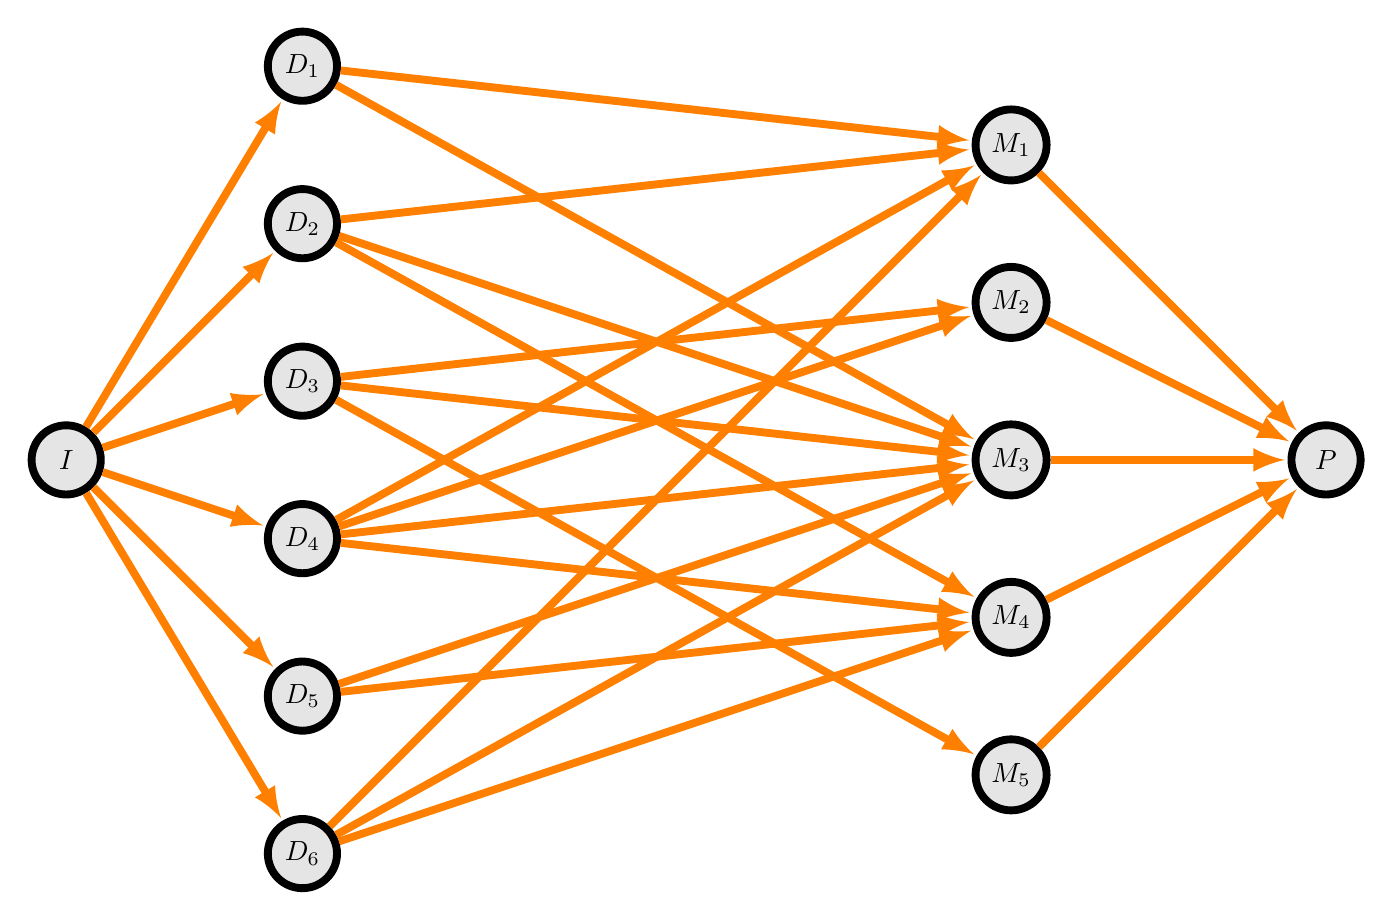
\begin{tikzpicture}[font=\sffamily]
        % Setup the style for the states
        \tikzset{node style/.style={state, 
                                    minimum width=0.5cm,
                                    line width=1mm,
                                    fill=gray!20!white}}
 
        % Draw the states
        \node[node style] at (3, 12) (masha1) {$D_1$};
        \node[node style] at (3,10) (masha2) {$D_2$};
        \node[node style] at (3,8) (masha3) {$D_3$};
        \node[node style] at (3,6) (masha4) {$D_4$};
        \node[node style] at (3,4) (masha5) {$D_5$};
        \node[node style] at (3,2) (masha6) {$D_6$};
        \node[node style] at (0,7) (izvor) {$I$};
        \node[node style] at (12, 11) (pasha1) {$M_1$};
        \node[node style] at (12,9) (pasha2) {$M_2$};
        \node[node style] at (12,7) (pasha3) {$M_3$};
        \node[node style] at (12,5) (pasha4) {$M_4$};
        \node[node style] at (12,3) (pasha5) {$M_5$};
        \node[node style] at (16,7) (ponor) {$P$};
        % Connect the states with arrows
        \draw[every loop,
              auto=right,
              line width=1mm,
              >=latex,
              draw=orange,
              fill=orange]
            (izvor)     edge[bend right=0]            node {} (masha1)
            (izvor)     edge[bend right=0]            node {} (masha2)
            (izvor)     edge[bend right=0]            node {} (masha3)
            (izvor)     edge[bend right=0]            node {} (masha4)
            (izvor)     edge[bend right=0]            node {} (masha5)
            (izvor)     edge[bend right=0]            node {} (masha6)
            (pasha1)     edge[bend right=0]            node {} (ponor)
            (pasha2)     edge[bend right=0]            node {} (ponor)
            (pasha3)     edge[bend right=0]            node {} (ponor)
            (pasha4)     edge[bend right=0]            node {} (ponor)
            (pasha5)     edge[bend right=0]            node {} (ponor)
            (masha1)     edge[bend right=0]            node {} (pasha1)
            (masha1)     edge[bend right=0]            node {} (pasha3)
            (masha2)     edge[bend right=0]            node {} (pasha1)
            (masha2)     edge[bend right=0]            node {} (pasha3)
            (masha2)     edge[bend right=0]            node {} (pasha4)
            (masha3)     edge[bend right=0]            node {} (pasha2)
            (masha3)     edge[bend right=0]            node {} (pasha3)
            (masha3)     edge[bend right=0]            node {} (pasha5)
            (masha4)     edge[bend right=0]            node {} (pasha1)
            (masha4)     edge[bend right=0]            node {} (pasha2)
            (masha4)     edge[bend right=0]            node {} (pasha3)
            (masha4)     edge[bend right=0]            node {} (pasha4)
            (masha5)     edge[bend right=0]            node {} (pasha3)
            (masha5)     edge[bend right=0]            node {} (pasha4)
            (masha6)     edge[bend right=0]            node {} (pasha1)
            (masha6)     edge[bend right=0]            node {} (pasha3)
            (masha6)     edge[bend right=0]            node {} (pasha4);
\end{tikzpicture}
\\
\\
\begin{tabular}{|c|c|c|c|c|c|}
\hline
      & $M_1$                    & $M_2$                    & $M_3$                    & $M_4$                    & $M_5$                    \\ \hline
$D_1$ & {\color[HTML]{000000} 1} & {\color[HTML]{000000} }  & {\color[HTML]{000000} 1} & {\color[HTML]{000000} }  & {\color[HTML]{000000} }  \\ \hline
$D_2$ & {\color[HTML]{000000} 1} & {\color[HTML]{000000} }  & {\color[HTML]{000000} 1} & {\color[HTML]{000000} 1} & {\color[HTML]{000000} }  \\ \hline
$D_3$ & {\color[HTML]{000000} }  & {\color[HTML]{FE0000} 1} & {\color[HTML]{FE0000} 1} & {\color[HTML]{000000} }  & {\color[HTML]{3166FF} 1} \\ \hline
$D_4$ & {\color[HTML]{000000} 1} & {\color[HTML]{000000} 1} & {\color[HTML]{000000} 1} & {\color[HTML]{000000} 1} & {\color[HTML]{000000} }  \\ \hline
$D_5$ & {\color[HTML]{000000} }  & {\color[HTML]{000000} }  & {\color[HTML]{000000} 1} & {\color[HTML]{000000} 1} & {\color[HTML]{000000} }  \\ \hline
$D_6$ & {\color[HTML]{000000} 1} & {\color[HTML]{000000} }  & {\color[HTML]{000000} 1} & {\color[HTML]{000000} 1} & {\color[HTML]{000000} }  \\ \hline
\end{tabular}
\begin{tabular}{|c|c|c|c|c|c|}
\hline
      & $M_1$                    & $M_2$                    & $M_3$                    & $M_4$                    & $M_5$                    \\ \hline
$D_1$ & {\color[HTML]{000000} 1} & {\color[HTML]{000000} }  & {\color[HTML]{000000} 1} & {\color[HTML]{000000} }  & {\color[HTML]{000000} }  \\ \hline
$D_2$ & {\color[HTML]{000000} 1} & {\color[HTML]{000000} }  & {\color[HTML]{000000} 1} & {\color[HTML]{000000} 1} & {\color[HTML]{000000} }  \\ \hline
$D_3$ & {\color[HTML]{000000} }  & {\color[HTML]{FE0000} 1} & {\color[HTML]{FE0000} 1} & {\color[HTML]{000000} }  & {\color[HTML]{3166FF} 1} \\ \hline
$D_4$ & {\color[HTML]{FE0000} 1} & {\color[HTML]{3166FF} 1} & {\color[HTML]{FE0000} 1} & {\color[HTML]{FE0000} 1} & {\color[HTML]{000000} }  \\ \hline
$D_5$ & {\color[HTML]{000000} }  & {\color[HTML]{000000} }  & {\color[HTML]{000000} 1} & {\color[HTML]{000000} 1} & {\color[HTML]{000000} }  \\ \hline
$D_6$ & {\color[HTML]{000000} 1} & {\color[HTML]{000000} }  & {\color[HTML]{000000} 1} & {\color[HTML]{000000} 1} & {\color[HTML]{000000} }  \\ \hline
\end{tabular}
\begin{tabular}{|c|c|c|c|c|c|}
\hline
      & $M_1$                    & $M_2$                    & $M_3$                    & $M_4$                    & $M_5$                    \\ \hline
$D_1$ & {\color[HTML]{3166FF} 1} & {\color[HTML]{000000} }  & {\color[HTML]{FE0000} 1} & {\color[HTML]{000000} }  & {\color[HTML]{000000} }  \\ \hline
$D_2$ & {\color[HTML]{FE0000} 1} & {\color[HTML]{000000} }  & {\color[HTML]{000000} 1} & {\color[HTML]{000000} 1} & {\color[HTML]{000000} }  \\ \hline
$D_3$ & {\color[HTML]{000000} }  & {\color[HTML]{FE0000} 1} & {\color[HTML]{FE0000} 1} & {\color[HTML]{000000} }  & {\color[HTML]{3166FF} 1} \\ \hline
$D_4$ & {\color[HTML]{FE0000} 1} & {\color[HTML]{3166FF} 1} & {\color[HTML]{FE0000} 1} & {\color[HTML]{FE0000} 1} & {\color[HTML]{000000} }  \\ \hline
$D_5$ & {\color[HTML]{000000} }  & {\color[HTML]{000000} }  & {\color[HTML]{000000} 1} & {\color[HTML]{000000} 1} & {\color[HTML]{000000} }  \\ \hline
$D_6$ & {\color[HTML]{FE0000} 1} & {\color[HTML]{000000} }  & {\color[HTML]{000000} 1} & {\color[HTML]{000000} 1} & {\color[HTML]{000000} }  \\ \hline
\end{tabular}\\
\\
\begin{tabular}{|c|c|c|c|c|c|}
\hline
      & $M_1$                    & $M_2$                    & $M_3$                    & $M_4$                    & $M_5$                    \\ \hline
$D_1$ & {\color[HTML]{3166FF} 1} & {\color[HTML]{000000} }  & {\color[HTML]{FE0000} 1} & {\color[HTML]{000000} }  & {\color[HTML]{000000} }  \\ \hline
$D_2$ & {\color[HTML]{FE0000} 1} & {\color[HTML]{000000} }  & {\color[HTML]{3166FF} 1} & {\color[HTML]{FE0000} 1} & {\color[HTML]{000000} }  \\ \hline
$D_3$ & {\color[HTML]{000000} }  & {\color[HTML]{FE0000} 1} & {\color[HTML]{FE0000} 1} & {\color[HTML]{000000} }  & {\color[HTML]{3166FF} 1} \\ \hline
$D_4$ & {\color[HTML]{FE0000} 1} & {\color[HTML]{3166FF} 1} & {\color[HTML]{FE0000} 1} & {\color[HTML]{FE0000} 1} & {\color[HTML]{000000} }  \\ \hline
$D_5$ & {\color[HTML]{000000} }  & {\color[HTML]{000000} }  & {\color[HTML]{FE0000} 1} & {\color[HTML]{000000} 1} & {\color[HTML]{000000} }  \\ \hline
$D_6$ & {\color[HTML]{FE0000} 1} & {\color[HTML]{000000} }  & {\color[HTML]{FE0000} 1} & {\color[HTML]{000000} 1} & {\color[HTML]{000000} }  \\ \hline
\end{tabular}
\begin{tabular}{|c|c|c|c|c|c|}
\hline
      & $M_1$                    & $M_2$                    & $M_3$                    & $M_4$                    & $M_5$                    \\ \hline
$D_1$ & {\color[HTML]{3166FF} 1} & {\color[HTML]{000000} }  & {\color[HTML]{FE0000} 1} & {\color[HTML]{000000} }  & {\color[HTML]{000000} }  \\ \hline
$D_2$ & {\color[HTML]{FE0000} 1} & {\color[HTML]{000000} }  & {\color[HTML]{3166FF} 1} & {\color[HTML]{FE0000} 1} & {\color[HTML]{000000} }  \\ \hline
$D_3$ & {\color[HTML]{000000} }  & {\color[HTML]{FE0000} 1} & {\color[HTML]{FE0000} 1} & {\color[HTML]{000000} }  & {\color[HTML]{3166FF} 1} \\ \hline
$D_4$ & {\color[HTML]{FE0000} 1} & {\color[HTML]{3166FF} 1} & {\color[HTML]{FE0000} 1} & {\color[HTML]{FE0000} 1} & {\color[HTML]{000000} }  \\ \hline
$D_5$ & {\color[HTML]{000000} }  & {\color[HTML]{000000} }  & {\color[HTML]{FE0000} 1} & {\color[HTML]{3166FF} 1} & {\color[HTML]{000000} }  \\ \hline
$D_6$ & {\color[HTML]{FE0000} 1} & {\color[HTML]{000000} }  & {\color[HTML]{FE0000} 1} & {\color[HTML]{FE0000} 1} & {\color[HTML]{000000} }  \\ \hline
\end{tabular}
\\
\\ \\
Po završetku ovog postupka očito je da je pronađeno maksimalno uparivanje, pri kojem je bez
partnera ostala djevojka $D_6$. Moralo se desiti da jedna od djevojaka ostane bez partnera pošto nije dozvoljeno da isti momak bude u vezi da više djevojaka odjednom, a prisutna je jedna više djevojka u odnosu na broj prisutnih momaka. Također je bitno primijetiti da je u moguće bilo dobiti nekoliko više različitih uparivanja, što znači da je dobijeni raspored samo jedan od više mogućih (sprovođenjem ovog postupka više puta uz pravljenje drugačijeg izbora pri uparivanju dovelo bi
do pronalaska svih mogućih rasporeda momaka i djevojaka). On
glasi:
\begin{equation*}
    D_1 - M_1 \quad D_2 - M_3 \quad D_3 - M_5 \quad D_4 - M_2 \quad D_5 - M_4 
\end{equation*}




\end{document}
